% =====================================================================
%  Práctica 3 · Identificación y caracterización de diodos LED
%  Instrumentación Electrónica · Grado en Física · USAL · 2026/2027
%  Compilar:  latexmk -pdf practica3_diodos_LED.tex
%  (los datos ilustrativos se regeneran con scripts/generar_datos.py)
% =====================================================================
\documentclass[11pt,a4paper]{article}
\usepackage{estilo}
\newcommand\pendienteajuste{1.10}
\newcommand\ordenadaajuste{-0.34}
\newcommand\umbralpn{0.63}
\newcommand\umbralzener{0.71}
\newcommand\tensionzener{3.27}
\newcommand\nshockley{1.91}
\newcommand\isshockley{3.3}

\CatchFileDef{\tablaumbral}{datos/tabla_umbral.tex}{}

\begin{document}

% =====================================================================
%                              PORTADA
% =====================================================================
\thispagestyle{empty}
\noindent\begin{tikzpicture}[remember picture,overlay]
  \shade[top color=azulclaro!70,bottom color=white]
    ($(current page.north west)+(0,-0.35)$) rectangle
    ($(current page.north east)+(0,-6.5)$);
  \shade[left color=navy,right color=azulmed!45,middle color=azul!85]
    (current page.north west) rectangle ($(current page.north east)+(0,-0.35)$);
  \shade[left color=navy,right color=azulmed!45,middle color=azul!85]
    (current page.south west) rectangle ($(current page.south east)+(0,0.35)$);
\end{tikzpicture}\par
\vspace*{-0.9cm}
\noindent
\begin{tabularx}{\linewidth}{@{}l>{\centering\arraybackslash}Xr@{}}
  \raisebox{-.5\height}{
\includegraphics[height=1.0cm]{img/logo-usal.png}} &
  \begin{tabular}{@{}c@{}}
    {\color{navy}\large\textls[120]{\textsc{Universidad de Salamanca}}}\\[2pt]
    {\color{grisazul}\small\textls[100]{\textsc{Facultad de Ciencias\ \ $\cdot$\ \ Grado en Física}}}
  \end{tabular} &
  \raisebox{-.5\height}{
\includegraphics[height=0.95cm]{img/logo-ciencias.png}}
\end{tabularx}
\par\vspace{6pt}
\noindent{\color{grisclaro}\rule{\linewidth}{.6pt}}
\vspace{0.7cm}

\noindent{\color{azul}\large\textls[150]{\textsc{Instrumentación Electrónica\ \ $\cdot$\ \ Práctica 3}}}
\par\vspace{0.35cm}
\noindent{\fontsize{30}{37}\selectfont\bfseries\color{navy}Identificación y
caracterización\\[2pt] de diodos LED\par}
\vspace{6pt}
\noindent\tikz\shade[left color=navy,right color=white,middle color=azul]
  (0,0) rectangle (0.5\linewidth,2.6pt);
\par\vspace{0.45cm}
\noindent{\large\itshape\color{black!80}
Unión pn, ecuación de Shockley y tensión umbral; diodo rectificador, diodo
Zener y LED de siete colores; montaje con el DAQ, instrumento virtual en
LabVIEW y lectura de la característica $\ID(\VD)$\par}
\vspace{0.6cm}

\noindent
\begin{minipage}[t]{0.5\linewidth}
  {\color{azul}\small\textls[120]{\textsc{Autor}}}\\[2pt]
  {\large Daniel Martín Guerrero\,\textsuperscript{a}}
\end{minipage}%
\begin{minipage}[t]{0.5\linewidth}
  {\color{azul}\small\textls[120]{\textsc{Asignatura}}}\\[2pt]
  {\large Instrumentación Electrónica\,\textsuperscript{a}}
\end{minipage}
\par\vspace{5pt}
\noindent{\small\color{grisazul}\textsuperscript{a}\,Grado en Física, Facultad de
Ciencias, Universidad de Salamanca, Plaza de la Merced s/n, 37008 Salamanca,
España\par}
\vspace{0.55cm}

\noindent
\begin{tcolorbox}[enhanced,sharp corners,boxrule=0pt,frame hidden,
  borderline west={2.2pt}{0pt}{navy},
  interior style={left color=azulclaro,right color=white},
  left=9pt,right=6pt,top=6pt,bottom=6pt,width=\linewidth]
\begin{minipage}[t]{0.585\linewidth}
  {\color{navy}\textls[120]{\textsc{Resumen}}}\par\vspace{4pt}
  \small\setlength{\parindent}{0pt}\linespread{1.12}\selectfont
  Esta guía prepara la práctica de caracterización de diodos con el sistema
  de adquisición (DAQ). Repasamos la física de la unión pn y de la emisión
  de luz en un LED, la simbología y cómo identificar ánodo y cátodo, y
  detallamos el circuito $R$--diodo que hay que montar, las conexiones
  AO-0/AI-1/GND y la configuración del instrumento virtual en LabVIEW. Se
  explica qué aparecerá en la gráfica $XY$ (la «oscilograma» $\ID$ frente a
  $\VD$) para cada componente y cómo extraer de ella la tensión umbral
  $\Vg$, la tensión Zener $\VZ$ y la relación $e\Vg\simeq hc/\lambda$ entre
  el color del LED y su umbral.
\end{minipage}\hfill
\begin{minipage}[t]{0.38\linewidth}\centering\vspace{2pt}
  % Figura de la portada: I-V de los LED (datos simulados)
\begin{tikzpicture}
\begin{axis}[width=5.9cm,height=4.6cm,
  xmin=0.6,xmax=3.4,ymin=-0.15,ymax=4.1,
  xlabel={$\VD$ (V)},ylabel={$\ID$ (mA)},
  xlabel style={font=\scriptsize,yshift=3pt},ylabel style={font=\scriptsize,yshift=-4pt},
  tick label style={font=\tiny},grid=major,
  axis background/.style={fill=white}]
  \foreach \col/\fic in {cIR/ir,cRojo/rojo,cAmarillo/amarillo,cVerde/verde,cAzul/azul,cUV/uv}{
    \edef\temp{\noexpand\addplot[\col,thick,mark=*,mark size=.7pt]
      table[x=VD,y=ID]{datos/iv_\fic.dat};}
    \temp}
\end{axis}
\end{tikzpicture}
\\[1pt]
  \parbox{0.95\linewidth}{\centering\scriptsize\color{grisazul}
  Característica $\ID(\VD)$ de LED de distintos colores: el umbral crece
  al disminuir la longitud de onda.}
\end{minipage}
\end{tcolorbox}
\vspace{0.25cm}

\noindent{\color{azul}\textls[120]{\textsc{Palabras clave}}}\ \
unión pn $\cdot$ ecuación de Shockley $\cdot$ tensión umbral $\cdot$ diodo
Zener $\cdot$ LED $\cdot$ banda prohibida $\cdot$ recta de carga $\cdot$ DAQ
$\cdot$ LabVIEW $\cdot$ característica $I$--$V$
\par\vspace{5pt}
\noindent{\color{azul}\textls[120]{\textsc{Clasificación PACS}}}\ \ 85.30.Kk
(diodos de unión); 85.60.Jb (dispositivos emisores de luz); 07.05.Hd
(adquisición de datos)
\par\vspace{7pt}{\color{grisclaro}\hrule height .5pt}\vspace{9pt}
\noindent\hfill
$\ID=\IS\bigl(e^{\VD/n\VT}-1\bigr)$\hfill
$\ID=\dfrac{\Vin-\VD}{R}$\hfill
$e\Vg\simeq\Eg\simeq\dfrac{hc}{\lambda}$\hfill
$\Vg[\si{V}]\simeq\dfrac{1240}{\lambda[\si{nm}]}$\hfill\null
\par\vspace{9pt}{\color{grisclaro}\hrule height .5pt}

\vfill
\begin{center}
  {\color{navy}\large\textls[150]{\textsc{Guía de laboratorio con fundamentos teóricos}}}\\[6pt]
  {\color{grisazul}\textls[120]{\textsc{Salamanca, curso 2026/2027}}}
\end{center}
\vspace*{0.2cm}
\newpage

% =====================================================================
\pagestyle{plain}
\renewcommand{\contentsname}{Índice}
{\hypersetup{linkcolor=black}\tableofcontents}
\newpage
\pagestyle{fancy}

% =====================================================================
\section{Introducción: qué vamos a hacer y por qué}
% =====================================================================

El diodo es el elemento no lineal más sencillo de la electrónica: deja pasar
la corriente en un sentido y la bloquea en el otro. Esa asimetría nace de la
física de la \emph{unión pn}, y en un tipo particular de diodo, el \emph{LED}
(\emph{light-emitting diode}), la energía que liberan los portadores al
recombinarse sale en forma de luz cuyo color está fijado por el material. En
esta práctica construiremos un pequeño \emph{trazador de curvas}: un
instrumento virtual que barre la tensión aplicada a un circuito, mide la
respuesta y dibuja la característica corriente--tensión $\ID(\VD)$ de cada
diodo~\cite{guion}.

Seguimos la estructura del guion de la práctica~\cite{guion}; la teoría de
semiconductores puede ampliarse en~\cite{sze,pierret}, la física de los LED
en~\cite{schubert} y los aspectos de circuito en~\cite{horowitz,sedra}.

\subsection{Objetivos}

\begin{enumerate}
  \item Caracterizar un \textbf{diodo pn} de silicio, un \textbf{diodo Zener}
        y \textbf{LED} de siete tipos: infrarrojo (IR), rojo, amarillo,
        verde, azul, blanco y ultravioleta (UV).
  \item Montar en la protoboard el circuito $R$--diodo y conectarlo al DAQ:
        la salida analógica \textbf{AO-0} impone $\Vin$ y la entrada
        analógica \textbf{AI-1} mide $\VD$.
  \item Programar en LabVIEW el barrido de $\Vin$, el cálculo de
        $\ID=(\Vin-\VD)/R$, la representación $XY$ y el guardado de los datos.
  \item Extraer la \textbf{tensión umbral} $\Vg$ de cada diodo, la
        \textbf{tensión Zener} $\VZ$ y explicar la dependencia de $\Vg$ con
        el color (longitud de onda) del LED.
\end{enumerate}

\Cref{fig:esquema-general} resume la cadena de medida y la
\cref{tab:magnitudes} lo que se impone, lo que se mide y lo que se calcula.

\begin{figure}[htbp]
  \centering
  % Cadena de medida: PC (LabVIEW) - DAQ - circuito
\begin{tikzpicture}[font=\small,
  bloque/.style={draw=#1,fill=#1!8,thick,rounded corners=3pt,align=center,
     minimum height=1.6cm,inner sep=5pt},
  flecha/.style={-{Stealth[length=6pt]},thick,#1},
  flecha/.default=grisazul]
  \node[bloque=navy,minimum width=3.3cm] (pc) at (0,0)
    {\textbf{PC}\\[-1pt]{\footnotesize LabVIEW}\\[-1pt]{\footnotesize rampa, cálculo, gráfica}};
  \node[bloque=azul,minimum width=2.6cm] (daq) at (5.0,0)
    {\textbf{DAQ}\\[-1pt]{\footnotesize myDAQ / Signal}\\[-1pt]{\footnotesize Accessory}};
  \node[bloque=ambar,minimum width=3.2cm,minimum height=2.3cm] (circ) at (10.1,0) {};
  \node[font=\footnotesize\bfseries,ambar!70!black,anchor=north] at (circ.north) {Protoboard};
  \begin{scope}[shift={(9.05,-0.55)},scale=0.62,transform shape]
    \draw (0,1.6) to[R] (1.8,1.6) to[leD*] (1.8,0) -- (0,0);
    \fill (1.8,1.6) circle (2pt);
  \end{scope}
  \draw[flecha] ([yshift=4pt]pc.east) -- node[above,font=\footnotesize]{$\Vin(k)$} ([yshift=4pt]daq.west);
  \draw[flecha] ([yshift=-8pt]daq.west) -- node[below,font=\footnotesize]{$\VD(k)$} ([yshift=-8pt]pc.east);
  \draw[flecha=rojoaviso] ([yshift=10pt]daq.east) -- node[above,font=\footnotesize\bfseries]{AO-0} ([yshift=10pt]circ.west);
  \draw[flecha=cAzul] ([yshift=-4pt]circ.west) -- node[below,font=\footnotesize\bfseries]{AI-1} ([yshift=-4pt]daq.east);
  \draw[black!70,thick] ([yshift=-22pt]daq.east) -- node[below,font=\footnotesize\bfseries]{GND} ([yshift=-22pt]circ.west);
  % salidas
  \node[draw=grisclaro,fill=white,rounded corners=2pt,align=center,font=\footnotesize] (graf) at (-0.9,-2.35)
    {gráfica $XY$\\$\ID$ vs.\ $\VD$};
  \node[draw=grisclaro,fill=white,rounded corners=2pt,align=center,font=\footnotesize] (fich) at (1.3,-2.35)
    {fichero\\ \ttt{.txt}};
  \draw[flecha] (pc.south) ++(-0.9,0) -- (graf.north);
  \draw[flecha] (pc.south) ++(1.3,0) -- (fich.north);
\end{tikzpicture}

  \caption{Cadena de medida de la práctica. El programa de LabVIEW genera una
  rampa de $N$ valores de $\Vin$ entre $V_{\text{start}}$ y $V_{\text{end}}$; en
  cada iteración el DAQ la impone en AO-0, espera, lee $\VD$ en AI-1, y el
  programa calcula $\ID$ por la ley de Ohm, añade el punto $(\VD,\ID)$ a la
  gráfica $XY$ y, al terminar, guarda todo en un fichero de texto.}
  \label{fig:esquema-general}
\end{figure}

\begin{table}[htbp]
  \centering\small
  \caption{Magnitudes de la práctica: qué fija el usuario, qué impone y mide
  el DAQ y qué se calcula.}
  \label{tab:magnitudes}
  \renewcommand{\arraystretch}{1.25}
  \begin{tabularx}{\linewidth}{@{}l l X l@{}}
    \toprule
    \textbf{Magnitud} & \textbf{Papel} & \textbf{Cómo se obtiene} & \textbf{Valor típico}\\
    \midrule
    $V_{\text{start}},\,V_{\text{end}}$ & control & Panel frontal (rango de la rampa) & $-5$ y $+5$\,V\\
    $N$ (\# muestras) & control & Panel frontal & $100$--$200$\\
    $R$ & control & Panel frontal (valor nominal, en k$\Omega$) & $1$\,k$\Omega$\\
    \rowcolor{azulpalido}
    $\Vin$ & impuesta & AO-0 del DAQ, un valor por iteración & $[-5,\,5]$\,V\\
    \rowcolor{azulpalido}
    $\VD$ & medida & AI-1 del DAQ (tensión ánodo--cátodo) & $[-5,\,3{,}3]$\,V\\
    $\ID$ & calculada & $\ID=(\Vin-\VD)/R$ & $[-5,\,4{,}5]$\,mA\\
    $\Vg,\ \VZ$ & resultado & Análisis de la curva $\ID(\VD)$ (\cref{sec:analisis}) & según diodo\\
    \bottomrule
  \end{tabularx}
\end{table}

% =====================================================================
\section{Fundamentos: la unión pn}
\label{sec:fundamentos}
% =====================================================================

\subsection{Semiconductores, bandas y dopado}

En un sólido cristalino los niveles de energía de los electrones se agrupan
en bandas. En un semiconductor la \emph{banda de valencia} (BV), llena a
$T=0$, y la \emph{banda de conducción} (BC), vacía, están separadas por una
\emph{banda prohibida} de anchura $\Eg$ de aproximadamente \SIrange{1}{3.5}{eV}.

\begin{definicion}{Banda prohibida y portadores}{gap}
  La \emph{energía de la banda prohibida} (\emph{gap}) es
  $\Eg=E_c-E_v$, diferencia entre el mínimo de la BC y el máximo de la BV.
  Los portadores de carga son los \emph{electrones} de la BC (carga $-e$) y
  los \emph{huecos} de la BV (estados vacíos que se comportan como cargas
  $+e$).
\end{definicion}

Añadiendo impurezas (\emph{dopado}) se controla qué portador domina: con
donadores (P, As en Si) se obtiene un semiconductor \textbf{tipo n}, con
mayoría de electrones; con aceptores (B, Al) uno \textbf{tipo p}, con
mayoría de huecos. Valores representativos: $\Eg(\text{Si})=\SI{1.12}{eV}$,
$\Eg(\text{GaAs})=\SI{1.42}{eV}$, $\Eg(\text{GaN})=\SI{3.4}{eV}$~\cite{sze}.

\subsection{La unión pn en equilibrio}

Al poner en contacto una región p y una n, los electrones difunden hacia p y
los huecos hacia n, donde se recombinan. Junto a la unión quedan los iones
fijos sin compensar: aparece una \emph{zona de carga espacial} (o \emph{de
deplexión}), sin portadores libres, con un campo eléctrico $\vec E$ dirigido
de n a p que frena la difusión (\cref{fig:union}). En equilibrio la difusión
y el arrastre se compensan y se establece una barrera de potencial
$V_{\text{bi}}$ (\emph{built-in}), del orden de $\Eg/e$.

\begin{figure}[htbp]
  \centering
  % Unión pn: estructura (a) y bandas en equilibrio (b)
\begin{tikzpicture}[font=\small,
  ion/.style={circle,draw=#1,inner sep=0pt,minimum size=9pt,font=\tiny\bfseries,text=#1},
  hueco/.style={circle,draw=cRojo!80!black,fill=white,inner sep=0pt,minimum size=4.5pt},
  electron/.style={circle,fill=cAzul,inner sep=0pt,minimum size=4.5pt}]
  % ---------------- (a) estructura
  \begin{scope}
    \fill[cRojo!12] (-4,0) rectangle (0,2.2);
    \fill[cAzul!12] (0,0) rectangle (4,2.2);
    \fill[pattern=north east lines,pattern color=grisclaro] (-1,0) rectangle (1,2.2);
    \fill[cRojo!22,opacity=.6] (-1,0) rectangle (0,2.2);
    \fill[cAzul!22,opacity=.6] (0,0) rectangle (1,2.2);
    \draw[grisazul,thick] (-4,0) rectangle (4,2.2);
    \draw[grisazul,dashed] (-1,0) -- (-1,2.2) (1,0) -- (1,2.2);
    \draw[navy,thick] (0,0) -- (0,2.2);
    \node[font=\bfseries\large,cRojo!80!black] at (-3.3,1.85) {p};
    \node[font=\bfseries\large,cAzul!80!black] at (3.3,1.85) {n};
    % portadores mayoritarios
    \foreach \x/\y in {-3.6/0.5,-3.0/1.1,-2.4/0.4,-1.9/1.5,-2.8/1.7,-1.5/0.8,-3.5/1.4,-2.1/1.0}
      \node[hueco] at (\x,\y) {};
    \foreach \x/\y in {3.6/0.5,3.0/1.1,2.4/0.4,1.9/1.5,2.8/1.7,1.5/0.8,3.5/1.4,2.1/1.0}
      \node[electron] at (\x,\y) {};
    % iones
    \foreach \y in {0.35,0.85,1.35,1.85}{
      \node[ion=cRojo!70!black] at (-0.65,\y) {$-$};
      \node[ion=cRojo!70!black] at (-0.25,\y-0.2) {$-$};
      \node[ion=cAzul!70!black] at (0.65,\y) {$+$};
      \node[ion=cAzul!70!black] at (0.25,\y-0.2) {$+$};}
    \draw[-{Stealth[length=7pt]},very thick,navy] (0.9,2.55) -- node[above]{$\vec E$} (-0.9,2.55);
    \draw[{Stealth[length=4pt]}-{Stealth[length=4pt]},grisazul] (-1,-0.25) -- (1,-0.25) node[midway,below=3pt,font=\footnotesize,align=center]{zona de carga\\[-2pt]espacial, $W$};
    \node[font=\footnotesize,grisazul,align=center] at (-2.6,-0.3) {huecos \tikz\node[hueco]{};\ mayoritarios};
    \node[font=\footnotesize,grisazul,align=center] at (2.7,-0.3) {electrones \tikz\node[electron]{};\ mayoritarios};
    \node[font=\bfseries] at (-4.5,2.2) {(a)};
    % contactos
    \draw[thick] (-4,1.1) -- (-4.4,1.1) node[left]{A};
    \draw[thick] (4,1.1) -- (4.4,1.1) node[right]{K};
  \end{scope}
  % ---------------- (b) bandas en equilibrio
  \begin{scope}[yshift=-4.9cm]
    \def\B{0.9}\def\w{0.45}
    \fill[cRojo!8] (-4,-0.6) rectangle (-1,2.9);
    \fill[cAzul!8] (1,-0.6) rectangle (4,2.9);
    \draw[navy,very thick,domain=-4:4,samples=120] plot (\x,{1.2+\B*(1-tanh(\x/\w))/2});
    \draw[navy,very thick,domain=-4:4,samples=120] plot (\x,{0.0+\B*(1-tanh(\x/\w))/2});
    \draw[rojoaviso,thick,dashed] (-4,1.05) -- (4,1.05) node[pos=0.88,below,font=\footnotesize]{$E_F$};
    \node[right,navy] at (4,1.2) {$E_c$};
    \node[right,navy] at (4,0.0) {$E_v$};
    \draw[{Stealth[length=4pt]}-{Stealth[length=4pt]},grisazul] (-3.5,1.2+\B) -- node[right,font=\footnotesize]{$\Eg$} (-3.5,\B);
    \draw[{Stealth[length=4pt]}-{Stealth[length=4pt]},azul] (2.2,1.2) -- node[right,font=\footnotesize]{$eV_{\text{bi}}$} (2.2,1.2+\B);
    \draw[azul,densely dotted] (-0.5,1.2+\B) -- (2.4,1.2+\B);
    \foreach \x in {1.4,1.8,2.6,3.0,3.4,3.8} \node[electron] at (\x,1.32) {};
    \foreach \x in {-1.4,-1.8,-2.6,-3.0,-3.4,-3.8} \node[hueco] at (\x,\B-0.12) {};
    \draw[grisazul,-{Stealth[length=5pt]}] (-4.1,-0.6) -- (-4.1,3.0) node[above,font=\footnotesize]{$E$};
    \draw[grisazul,-{Stealth[length=5pt]}] (-4.1,-0.6) -- (4.6,-0.6) node[right,font=\footnotesize]{$x$};
    \node[font=\bfseries] at (-4.5,2.9) {(b)};
    \node[cRojo!80!black,font=\footnotesize] at (-2.5,2.65) {lado p};
    \node[cAzul!80!black,font=\footnotesize] at (2.5,2.65) {lado n};
  \end{scope}
\end{tikzpicture}

  \caption{(a) Unión pn en equilibrio: la difusión de portadores deja una zona
  de carga espacial de anchura $W$ con iones aceptores ($\ominus$) en el lado p
  e iones donadores ($\oplus$) en el lado n, que crean un campo $\vec E$ de n
  a p. (b) Diagrama de bandas: el nivel de Fermi $E_F$ es constante y las
  bandas se curvan en la zona de carga espacial formando la barrera
  $eV_{\text{bi}}$.}
  \label{fig:union}
\end{figure}

\subsection{Polarización directa e inversa}

Aplicar una tensión $\VD$ entre ánodo (p) y cátodo (n) modifica la barrera
(\cref{fig:bandas}):
\begin{itemize}
  \item \textbf{Directa} ($\VD>0$): la barrera baja a $e(V_{\text{bi}}-\VD)$;
    una fracción exponencialmente creciente de portadores la supera, se
    \emph{inyecta} en la región opuesta y se recombina. La corriente crece
    exponencialmente.
  \item \textbf{Inversa} ($\VD<0$): la barrera sube a
    $e(V_{\text{bi}}+|\VD|)$ y la zona de carga espacial se ensancha. Solo
    circula la diminuta corriente de saturación $-\IS$ (pA--nA), debida a los
    portadores minoritarios.
\end{itemize}

\begin{figure}[htbp]
  \centering
  % Diagramas de bandas: equilibrio, directa, inversa
\begin{tikzpicture}[font=\footnotesize,
  hueco/.style={circle,draw=cRojo!80!black,fill=white,inner sep=0pt,minimum size=4pt},
  electron/.style={circle,fill=cAzul,inner sep=0pt,minimum size=4pt},
  foton/.style={decorate,decoration={snake,amplitude=1.6pt,segment length=5pt,post length=4pt},
     -{Stealth[length=5pt]},cVerde!70!black,thick}]
  % #1 desplazamiento x, #2 barrera B, #3 E_Fp (lado p), #4 título, #5 etiqueta
  \newcommand{\panelbandas}[5]{%
  \begin{scope}[xshift=#1cm]
    \fill[cRojo!7] (-2.1,-0.35) rectangle (-0.45,2.75);
    \fill[cAzul!7] (0.45,-0.35) rectangle (2.1,2.75);
    \draw[navy,very thick,domain=-2.1:2.1,samples=80] plot (\x,{1.2+#2*(1-tanh(\x/0.3))/2});
    \draw[navy,very thick,domain=-2.1:2.1,samples=80] plot (\x,{#2*(1-tanh(\x/0.3))/2});
    \draw[rojoaviso,thick,dashed] (-2.1,#3) -- (0.35,#3);
    \draw[cAzul!80!black,thick,dashed] (-0.35,1.05) -- (2.1,1.05);
    \foreach \x in {0.9,1.25,1.6,1.95} \node[electron] at (\x,1.3) {};
    \foreach \x in {-0.9,-1.25,-1.6,-1.95} \node[hueco] at (\x,#2-0.1) {};
    \node[font=\bfseries] at (-1.85,2.95) {#5};
    \node[navy,align=center] at (0,3.05) {#4};
  \end{scope}}
  \panelbandas{0}{0.9}{1.05}{Equilibrio}{(a)}
  \panelbandas{5}{0.4}{0.55}{Directa, $\VD>0$}{(b)}
  \panelbandas{10}{1.4}{1.55}{Inversa, $\VD<0$}{(c)}
  % (a) etiquetas
  \node[navy,right] at (2.1,1.2) {$E_c$};
  \node[navy,right] at (2.1,0) {$E_v$};
  \node[rojoaviso,above] at (-1.3,1.05) {$E_F$};
  \draw[{Stealth[length=3.5pt]}-{Stealth[length=3.5pt]},azul] (1.2,1.25+0.0) ++(0,0.1) -- (1.2,2.1)
     node[midway,right]{$eV_{\text{bi}}$};
  % (b) directa
  \begin{scope}[xshift=5cm]
    \node[rojoaviso,left] at (-2.1,0.55) {$E_{Fp}$};
    \node[cAzul!80!black,above] at (1.5,1.4) {$E_{Fn}$};
    \draw[{Stealth[length=3.5pt]}-{Stealth[length=3.5pt]},grisazul] (-0.7,0.55) -- (-0.7,1.05)
       node[midway,left,font=\scriptsize]{$e\VD$};
    \draw[grisazul,densely dotted] (-0.7,1.05) -- (-0.35,1.05);
    % electrón inyectado que se recombina
    \node[electron] (e1) at (-0.15,1.45) {};
    \node[hueco] (h1) at (-0.15,0.33) {};
    \draw[-{Stealth[length=4pt]},cAzul,thick] (0.75,1.3) to[bend right=25] (e1);
    \draw[-{Stealth[length=4pt]},black!70,thick] (e1) -- (h1);
    \draw[foton] (-0.05,0.9) -- (1.4,0.35) node[right,cVerde!50!black]{$h\nu\simeq\Eg$};
  \end{scope}
  % (c) inversa
  \begin{scope}[xshift=10cm]
    \node[rojoaviso,above] at (-1.3,1.55) {$E_{Fp}$};
    \node[cAzul!80!black,below] at (1.5,1.0) {$E_{Fn}$};
    \draw[{Stealth[length=3.5pt]}-{Stealth[length=3.5pt]},azul] (1.0,1.3) -- (1.0,2.55)
       node[midway,right]{$e(V_{\text{bi}}+|\VD|)$};
  \end{scope}
\end{tikzpicture}

  \caption{Diagramas de bandas de la unión pn. (a) Equilibrio: $E_F$ único.
  (b) Polarización directa: la barrera se reduce, los cuasi-niveles de Fermi
  $E_{Fn}$ y $E_{Fp}$ se separan $e\VD$ y los electrones inyectados se
  recombinan con huecos; en un semiconductor de gap directo la energía sale
  como un fotón $h\nu\simeq\Eg$. (c) Polarización inversa: la barrera crece y
  la corriente es despreciable.}
  \label{fig:bandas}
\end{figure}

\subsection{Ecuación de Shockley y tensión umbral}

\begin{proposicion}{Ecuación del diodo de Shockley~\cite{shockley}}{shockley}
  La corriente de un diodo de unión ideal en función de la tensión aplicada es
  \begin{destacada}
    \ID=\IS\left(e^{\VD/n\VT}-1\right),\qquad \VT=\frac{k_BT}{e}\simeq\SI{25.9}{mV}\ (T=\SI{300}{K}),
    \label{eq:shockley}
  \end{destacada}
  donde $\IS$ es la corriente de saturación inversa y $n\in[1,2]$ el
  \emph{factor de idealidad}.
\end{proposicion}

En directa, en cuanto $\VD\gg n\VT$, la exponencial domina:
$\ln\ID\simeq\ln\IS+\VD/n\VT$, una recta en escala semilogarítmica
(\cref{fig:semilog}) de cuya pendiente se obtiene $n$. Por cada década de
corriente la tensión solo aumenta $n\VT\ln10\approx\SIrange{60}{120}{mV}$:
vista en escala lineal, la curva parece «apagada» hasta cierta tensión y
luego casi vertical. Ese codo define el parámetro práctico más importante.

\begin{definicion}{Tensión umbral}{umbral}
  La \emph{tensión umbral} (de codo o de encendido) $\Vg$ es la tensión a
  partir de la cual el diodo conduce de forma apreciable. Operativamente, en
  esta práctica la definimos como la intersección con el eje $\ID=0$ de la
  recta que ajusta el tramo de alta corriente de la característica
  $\ID(\VD)$ (\cref{fig:metodo-umbral}).
\end{definicion}

\begin{observacion}[Valores típicos]
  $\Vg\approx\SIrange{0.6}{0.7}{V}$ para un diodo de silicio,
  $\approx\SI{0.3}{V}$ para uno de germanio o Schottky, y entre
  $\approx\SI{1.1}{V}$ (LED IR) y $\approx\SI{3}{V}$ (LED UV) para los LED. Que
  $\Vg$ no es un valor «exacto» se ve en~\eqref{eq:shockley}: depende del rango
  de corriente usado para definir el codo y de la temperatura
  ($\mathrm d\Vg/\mathrm dT\approx\SI{-2}{mV/K}$).
\end{observacion}

\begin{figure}[htbp]
  \centering
  \begin{subfigure}[b]{0.49\linewidth}\centering
    \begin{tikzpicture}
\begin{axis}[width=7.4cm,height=6cm,ymode=log,
  xmin=0.3,xmax=0.75,ymin=3e-3,ymax=10,
  xlabel={$\VD$ (V)},ylabel={$\ID$ (mA)},grid=major,
  legend pos=north west,
  yticklabel style={/pgf/number format/fixed}]
  \addplot[azulmed,thick] table[x=VD,y=ID]{datos/semilog_fit.dat};
  \addlegendentry{Shockley, $n=\nshockley$}
  \addplot[medida,cPN] table[x=VD,y=ID]{datos/semilog_pn.dat};
  \addlegendentry{datos}
  \node[font=\scriptsize,azul,rotate=38,anchor=south] at (axis cs:0.45,0.06)
    {pendiente $1/(n\VT)$};
  \node[font=\scriptsize,grisazul,align=center,anchor=north] at (axis cs:0.66,0.9)
    {caída en\\[-2pt]$\Rs$};
\end{axis}
\end{tikzpicture}

    \caption{Escala semilogarítmica.}
    \label{fig:semilog}
  \end{subfigure}\hfill
  \begin{subfigure}[b]{0.49\linewidth}\centering
    \begin{tikzpicture}
\begin{axis}[width=7.4cm,height=6cm,
  xmin=-0.2,xmax=0.85,ymin=-0.3,ymax=4.8,
  xlabel={$\VD$ (V)},ylabel={$\ID$ (mA)},grid=major,
  legend style={at={(0.03,0.62)},anchor=west}]
  \fill[azulclaro,opacity=.8] (axis cs:0.55,2.15) rectangle (axis cs:0.8,4.5);
  \addplot[medida,cPN] table[x=VD,y=ID]{datos/iv_pn.dat};
  \addlegendentry{datos}
  \addplot[azul,thick,dashed,domain=0:1] table[x=VD,y=ID]{datos/fit_pn.dat};
  \addlegendentry{ajuste $\ID>I_{\max}/2$}
  \draw[black!60] (axis cs:-0.2,0) -- (axis cs:0.85,0);
  \fill[rojoaviso] (axis cs:\umbralpn,0) circle (1.8pt);
  \draw[rojoaviso,-{Stealth[length=5pt]}] (axis cs:0.25,1.0)
    node[above,font=\small]{$\Vg\simeq\SI{\umbralpn}{V}$} -- (axis cs:0.6,0.07);
\end{axis}
\end{tikzpicture}

    \caption{Escala lineal y método del umbral.}
    \label{fig:metodo-umbral}
  \end{subfigure}
  \caption{Característica directa del diodo pn (datos simulados con el
  circuito de la práctica). (a) En escala semilogarítmica el tramo
  exponencial es una recta; el ajuste de Shockley da $n\simeq\num{\nshockley}$ e
  $\IS\simeq\SI{\isshockley}{nA}$. A corrientes altas la caída en la
  resistencia serie curva los datos hacia abajo. (b) En escala lineal, la recta
  que ajusta el tramo de alta corriente corta el eje en
  $\Vg\simeq\SI{\umbralpn}{V}$.}
  \label{fig:shockley}
\end{figure}

\subsection{Modelos lineales por tramos}

Para analizar circuitos se sustituye~\eqref{eq:shockley} por modelos más
sencillos (\cref{fig:modelos}): el \emph{diodo ideal} (cortocircuito en
directa, circuito abierto en inversa), el modelo de \emph{tensión umbral}
(fuente $\Vg$ en directa) y el de \emph{umbral más resistencia dinámica}
$r_d=\mathrm d\VD/\mathrm d\ID\simeq n\VT/\ID$. Con $\ID\sim\SI{3}{mA}$,
$r_d\sim\SI{15}{\ohm}$, despreciable frente a $R=\SI{1}{k\ohm}$.

\begin{figure}[htbp]
  \centering
  % Modelos lineales por tramos del diodo
\begin{tikzpicture}[font=\footnotesize,
  ejes/.style={-{Stealth[length=4pt]},grisazul},
  real/.style={grisclaro,line width=2.2pt},
  modelo/.style={azul,very thick}]
  \newcommand{\ejesmodelo}[2]{%
    \draw[ejes] (-1.6,0) -- (2.3,0) node[below left]{$\VD$};
    \draw[ejes] (0,-0.4) -- (0,2.6) node[left]{$\ID$};
    \draw[real,domain=-1.6:1.33,samples=60] plot (\x,{0.0006*exp(\x/0.16)});
    \node[font=\bfseries] at (-1.4,2.5) {#1};
    \node[navy] at (0.4,-0.75) {#2};}
  \begin{scope}
    \ejesmodelo{(a)}{Ideal}
    \draw[modelo] (-1.6,0) -- (0,0) -- (0,2.4);
  \end{scope}
  \begin{scope}[xshift=4.6cm]
    \ejesmodelo{(b)}{Tensión umbral}
    \draw[modelo] (-1.6,0) -- (1.2,0) -- (1.2,2.4);
    \draw[grisazul,densely dotted] (1.2,0) -- (1.2,-0.15) node[below]{$\Vg$};
  \end{scope}
  \begin{scope}[xshift=9.2cm]
    \ejesmodelo{(c)}{Umbral $+\,r_d$}
    \draw[modelo] (-1.6,0) -- (1.1,0) -- (1.5,2.4);
    \draw[grisazul,densely dotted] (1.1,0) -- (1.1,-0.15) node[below]{$\Vg$};
    \draw[grisazul] (1.3,1.2) -- (1.7,1.2) node[right]{pendiente $1/r_d$};
  \end{scope}
\end{tikzpicture}

  \caption{Modelos del diodo: (a) ideal, (b) tensión umbral constante,
  (c) umbral más resistencia dinámica $r_d$. En gris, la característica real.}
  \label{fig:modelos}
\end{figure}

\subsection{Ruptura inversa: el diodo Zener}

Si la polarización inversa supera cierto valor, la corriente inversa crece
bruscamente: es la \emph{ruptura}. En diodos muy dopados el campo en la zona
de carga espacial es tan intenso que los electrones atraviesan la banda
prohibida por \emph{efecto túnel} (efecto Zener, $\VZ\lesssim\SI{5}{V}$); en
diodos menos dopados domina la \emph{multiplicación por avalancha}
($\VZ\gtrsim\SI{7}{V}$)~\cite{sze}. Un diodo normal no debe trabajar en
ruptura, pero el \textbf{diodo Zener} se fabrica para hacerlo de forma
controlada y reversible.

\begin{definicion}{Tensión Zener}{zener}
  La \emph{tensión Zener} $\VZ$ es el valor absoluto de la tensión inversa a
  la que el diodo entra en ruptura; en esa región $\VD\simeq-\VZ$
  prácticamente con independencia de la corriente. Por eso el Zener se usa
  como \emph{referencia} o \emph{regulador} de tensión.
\end{definicion}

\begin{observacion}[Rango del DAQ]
  El DAQ genera como mucho $|\Vin|=\SI{5}{V}$, y con $R=\SI{1}{k\ohm}$ la
  corriente inversa es $(|\Vin|-\VZ)/R$. Solo veremos la ruptura si
  $\VZ<\SI{5}{V}$ (por ejemplo, un Zener de \SI{3.3}{V} o \SI{4.7}{V}); para
  $\VZ$ mayores la rama inversa del Zener será idéntica a la de un diodo
  normal.
\end{observacion}

% =====================================================================
\section{Clases de diodos y simbología}
\label{sec:simbologia}
% =====================================================================

\subsection{Símbolos}

Todos los símbolos de diodo comparten un triángulo, que apunta en el
\emph{sentido convencional de la corriente directa}, y una barra, que
representa el \textbf{cátodo} (K, terminal $-$). El ánodo (A, terminal $+$)
está en la base del triángulo. Las variantes modifican la barra o añaden
flechas (\cref{tab:simbolos}).

\begin{table}[htbp]
  \centering\small
  \caption{Símbolos normalizados de los diodos más comunes. En todos, la
  corriente directa entra por el ánodo A y sale por el cátodo K. En esta
  práctica se usan los tres primeros.}
  \label{tab:simbolos}
  % Tabla de símbolos de diodos (circuitikz)
\newcommand{\simbolo}[1]{%
  \raisebox{-0.42\height}{\begin{circuitikz}[scale=0.85,transform shape,font=\scriptsize]
    \draw (0,0) node[left,azul]{A} to[#1] (2.2,0) node[right,azul]{K};
  \end{circuitikz}}}
\renewcommand{\arraystretch}{2.05}
\begin{tabularx}{\linewidth}{@{}c l X c@{}}
  \toprule
  \textbf{Símbolo} & \textbf{Tipo} & \textbf{Funcionamiento y uso} & \textbf{Parámetro}\\
  \midrule
  \rowcolor{azulpalido}
  \simbolo{D*} & Rectificador / señal & Unión pn de Si; rectificación, protección & $\Vg\approx\SI{0.6}{V}$\\
  \rowcolor{azulpalido}
  \simbolo{zD*} & Zener & Trabaja en ruptura inversa; referencia de tensión & $\VZ$\\
  \rowcolor{azulpalido}
  \simbolo{leD*} & LED & Emite luz en directa (flechas salientes) & $\Vg\simeq hc/e\lambda$\\
  \simbolo{pD*} & Fotodiodo & Genera corriente al absorber luz (flechas entrantes) & $I_{\text{luz}}$\\
  \simbolo{sD*} & Schottky & Unión metal--semiconductor; rápido & $\Vg\approx\SI{0.3}{V}$\\
  \simbolo{VC*} & Varicap & Capacidad dependiente de la tensión inversa & $C(\VD)$\\
  \bottomrule
\end{tabularx}

\end{table}

\subsection{Identificación física de ánodo y cátodo}

En el laboratorio no hay símbolos, sino componentes. La
\cref{fig:encapsulados} muestra cómo reconocer la polaridad en los
encapsulados que vamos a usar.

\begin{figure}[htbp]
  \centering
  % Encapsulados: diodo axial, diodo de vidrio, anatomía del LED, vista superior
\begin{tikzpicture}[font=\footnotesize,
  pata/.style={fill=gray!45,draw=gray!70!black,line width=.4pt},
  etiq/.style={grisazul,font=\scriptsize,align=left},
  guia/.style={grisazul!80,line width=.35pt}]
  % ================= (a) diodo axial de plástico
  \begin{scope}[shift={(0,3.0)}]
    \node[font=\bfseries\small] at (-1.9,0.75) {(a)};
    \draw[gray!60!black,line width=1.2pt] (-1.9,0) -- (1.9,0);
    \shade[top color=gray!55!black,bottom color=black!90,middle color=gray!70!black,
      rounded corners=2pt] (-0.75,-0.3) rectangle (0.75,0.3);
    \shade[top color=gray!15,bottom color=gray!55,middle color=white]
      (0.38,-0.3) rectangle (0.55,0.3);
    \node[azul,font=\small\bfseries] at (-1.7,-0.35) {A};
    \node[azul,font=\small\bfseries] at (1.7,-0.35) {K};
    \node[etiq,anchor=north] at (0.46,-0.35) {banda = cátodo};
    \node[grisazul,font=\scriptsize] at (0,0.55) {1N4007 (DO-41)};
  \end{scope}
  % ================= (b) diodo de vidrio
  \begin{scope}[shift={(0,1.0)}]
    \node[font=\bfseries\small] at (-1.9,0.75) {(b)};
    \draw[gray!60!black,line width=1pt] (-1.9,0) -- (1.9,0);
    \shade[top color=orange!35,bottom color=orange!70!brown,middle color=orange!15,
      rounded corners=4pt,opacity=.9] (-0.6,-0.22) rectangle (0.6,0.22);
    \draw[gray!60!black,line width=.8pt] (-0.45,0) -- (0.3,0);
    \fill[black!85] (0.32,-0.22) rectangle (0.45,0.22);
    \node[azul,font=\small\bfseries] at (-1.7,-0.35) {A};
    \node[azul,font=\small\bfseries] at (1.7,-0.35) {K};
    \node[etiq,anchor=north] at (0.39,-0.3) {banda = cátodo};
    \node[grisazul,font=\scriptsize] at (0,0.5) {1N4148 / Zener (DO-35)};
    % símbolo bajo los encapsulados
    \draw (-1.1,-2.1) node[left,azul]{A} to[D*] (1.1,-2.1) node[right,azul]{K};
    \draw[-{Stealth[length=5pt]},rojoaviso,thick] (-0.7,-1.5) -- node[above,font=\scriptsize]{corriente directa} (0.7,-1.5);
  \end{scope}
  % ================= (c) anatomía del LED
  \begin{scope}[shift={(6.4,-0.4)},scale=1.25]
    \node[font=\bfseries\small] at (-2.9,3.5) {(c)};
    % patillas
    \fill[pata] (-0.55,-2.9) rectangle (-0.37,0.05);
    \fill[pata] (0.37,-2.3) rectangle (0.55,0.05);
    % electrodos internos
    \fill[pata] (-0.55,0) -- (-0.55,1.55) -- (-0.3,1.78) -- (-0.12,1.78)
       -- (-0.12,1.48) -- (-0.37,1.36) -- (-0.37,0) -- cycle;
    \fill[pata] (-0.05,0.85) -- (-0.05,1.65) -- (0.08,1.65) -- (0.2,1.3)
       -- (0.55,1.3) -- (0.67,1.65) -- (0.85,1.65) -- (0.85,0.85) -- (0.55,0.85)
       -- (0.55,0) -- (0.37,0) -- (0.37,0.85) -- cycle;
    \fill[black!80] (0.31,1.3) rectangle (0.44,1.42);
    \draw[Goldenrod!80!black,line width=.5pt] (0.375,1.42) .. controls (0.35,2.0) and (-0.1,2.05) .. (-0.21,1.77);
    % rayos de luz
    \foreach \a in {60,75,90,105,120}
      \draw[cRojo,-{Stealth[length=3pt]},line width=.5pt] (0.375,1.5)++(\a:0.25) -- ++(\a:0.95);
    % cuerpo de epoxi
    \fill[cRojo!30,opacity=.45] (-1,0.3) -- (-1,2.3) arc (180:0:1) -- (1,0.3) -- cycle;
    \draw[cRojo!70!black,line width=.6pt] (-1,0.3) -- (-1,2.3) arc (180:0:1) -- (1,0.3);
    \fill[cRojo!45,opacity=.6] (-1.18,0) rectangle (1.02,0.3);
    \draw[cRojo!70!black,line width=.6pt] (-1.18,0) rectangle (1.02,0.3);
    % etiquetas izquierda
    \draw[guia] (-0.75,2.9) -- (-1.35,3.1) node[left,etiq]{lente de epoxi};
    \draw[guia] (0.0,1.97) -- (-1.35,2.45) node[left,etiq]{hilo de conexión};
    \draw[guia] (-0.47,1.2) -- (-1.35,1.5) node[left,etiq]{poste:\\ ánodo (A)};
    \draw[guia] (-0.46,-1.5) -- (-1.0,-1.5) node[left,etiq]{patilla larga\\ ánodo ($+$)};
    % etiquetas derecha
    \draw[guia] (0.4,1.36) -- (1.35,2.7) node[right,etiq]{chip (unión pn)};
    \draw[guia] (0.62,1.5) -- (1.35,2.05) node[right,etiq]{copa reflectora};
    \draw[guia] (0.75,1.0) -- (1.35,1.25) node[right,etiq]{yunque:\\ cátodo (K)};
    \draw[guia] (1.02,0.15) -- (1.35,0.35) node[right,etiq]{borde plano\\ = cátodo};
    \draw[guia] (0.46,-1.2) -- (1.0,-1.2) node[right,etiq]{patilla corta\\ cátodo ($-$)};
  \end{scope}
  % ================= (d) vista superior y símbolo
  \begin{scope}[shift={(12.4,1.6)}]
    \node[font=\bfseries\small] at (-1.0,1.7) {(d)};
    \begin{scope}
      \clip (-1,-1) rectangle (0.82,1);
      \fill[cRojo!35] (0,0) circle (0.95);
      \draw[cRojo!70!black] (0,0) circle (0.95);
    \end{scope}
    \draw[cRojo!70!black] (0.82,-0.47) -- (0.82,0.47);
    \fill[cRojo!20] (0,0) circle (0.7);
    \draw[cRojo!60!black] (0,0) circle (0.7);
    \node[etiq] at (0,-1.25) {vista superior};
    \draw[guia] (0.82,0.25) -- (1.2,0.6) node[above,etiq]{plano};
    \draw (0,-2.0) node[above right=-1pt,font=\scriptsize\bfseries,azul]{\,$+$} node[left,azul]{A}
       to[leD*] (0,-3.9) node[left,azul]{K} node[below right=-1pt,font=\scriptsize\bfseries,azul]{\,$-$};
  \end{scope}
\end{tikzpicture}

  \caption{Encapsulados de la práctica. (a) Diodo rectificador en encapsulado
  axial de plástico (p.\,ej.\ 1N4007): la \emph{banda} marca el cátodo. (b)
  Diodo de señal o Zener en vidrio (p.\,ej.\ 1N4148, BZX55): de nuevo la
  banda negra es el cátodo. (c) Anatomía de un LED de \SI{5}{mm}: el chip
  semiconductor descansa en la copa reflectora del \emph{yunque} (cátodo) y un
  hilo de oro lo une al \emph{poste} (ánodo); la patilla larga es el ánodo y
  el borde plano de la base señala el cátodo. (d) Vista superior y símbolo.}
  \label{fig:encapsulados}
\end{figure}

\begin{laboratorio}{Cómo identificar la polaridad}{polaridad}
  \begin{itemize}[leftmargin=1.2em]
    \item \textbf{Diodos axiales:} la banda (blanca, gris o negra) está en el
      lado del \textbf{cátodo}, igual que la barra del símbolo.
    \item \textbf{LED:} la \textbf{patilla larga es el ánodo} ($+$); la corta
      y el \textbf{borde plano} de la base indican el cátodo ($-$). Si las
      patillas se han cortado, el electrodo interior más grande (yunque)
      suele ser el cátodo, aunque no es universal.
    \item \textbf{Comprobación:} el modo «diodo» del multímetro
      (\raisebox{-1pt}{\tikz[scale=.3]{\draw[fill=black](0,0)--(0,.6)--(.6,.3)--cycle;\draw[thick](.6,0)--(.6,.6);}})
      marca $\approx\SI{0.6}{V}$ con la punta roja en el ánodo de un diodo de
      Si y enciende débilmente la mayoría de LED; en inversa marca «OL».
  \end{itemize}
\end{laboratorio}

% =====================================================================
\section{El LED: de la unión pn a la luz}
\label{sec:led}
% =====================================================================

\subsection{Recombinación radiativa}

Cuando en polarización directa un electrón de la BC se recombina con un hueco
de la BV, libera una energía $\approx\Eg$. En el silicio, de \emph{gap
indirecto}, la conservación del momento exige la participación de un fonón y
la energía acaba casi toda como calor. En semiconductores de \emph{gap
directo} (GaAs, AlGaInP, InGaN\ldots) la recombinación es mayoritariamente
\emph{radiativa}: se emite un fotón (\cref{fig:bandas}b).

\begin{proposicion}{Color y tensión umbral}{color}
  La energía de los fotones emitidos es $h\nu\simeq\Eg$, luego la longitud de
  onda del pico de emisión es
  \begin{destacada}
    \lambda\simeq\frac{hc}{\Eg},\qquad
    \lambda[\si{nm}]\simeq\frac{1240}{\Eg[\si{eV}]}.
    \label{eq:lambda}
  \end{destacada}
  Como para que circule corriente apreciable hay que reducir la barrera, que es
  del orden de $\Eg/e$, la tensión umbral cumple
  \begin{destacada}
    e\Vg\simeq\Eg\simeq\frac{hc}{\lambda}
    \quad\Longrightarrow\quad
    \Vg[\si{V}]\simeq\frac{1240}{\lambda[\si{nm}]}.
    \label{eq:umbral-lambda}
  \end{destacada}
\end{proposicion}

Así, \textbf{cuanto menor es la longitud de onda (más hacia el azul y el
violeta), mayor es la tensión umbral}: el LED IR enciende a $\approx\SI{1.1}{V}$
y el UV a $\approx\SI{3}{V}$. Es el resultado central que debéis explicar en
el informe y permite incluso \emph{estimar la constante de Planck}
(\cref{sec:planck}).

\subsection{Materiales y espectros}

El color se elige con el material y su composición (\cref{tab:leds}): GaAs
para el infrarrojo, AlGaInP para rojo--ámbar y InGaN para verde, azul y UV.
El \textbf{LED blanco} no existe como tal: es un chip azul de InGaN cubierto
de un \emph{fósforo} (YAG:Ce) que absorbe parte del azul y reemite en el
amarillo; su umbral es, por tanto, el de un LED azul. Los espectros
(\cref{fig:espectros}) son bandas de anchura \SIrange{15}{50}{nm}, no
líneas.

\begin{table}[htbp]
  \centering\small
  \caption{LED de la práctica: material típico, longitud de onda de pico,
  energía del fotón $E_{\text{ph}}=hc/\lambda_p$ y rango orientativo de
  $\Vg$. Los valores concretos dependen del fabricante: consultad la hoja de
  características.}
  \label{tab:leds}
  \renewcommand{\arraystretch}{1.2}
  \begin{tabular}{@{}l l c c c l@{}}
    \toprule
    \textbf{LED} & \textbf{Material} & $\lambda_p$ (nm) & $E_{\text{ph}}$ (eV)
      & $\Vg$ esperado (V) & \textbf{Observaciones}\\
    \midrule
    {\color{cIR}\rule{1.4ex}{1.4ex}}\ IR       & GaAs        & 940 & 1,32 & 1,0--1,2 & invisible; se ve con la cámara del móvil\\
    {\color{cRojo}\rule{1.4ex}{1.4ex}}\ Rojo     & AlGaInP     & 630 & 1,97 & 1,6--1,8 & \\
    {\color{cAmarillo}\rule{1.4ex}{1.4ex}}\ Amarillo & AlGaInP     & 590 & 2,10 & 1,7--1,9 & \\
    {\color{cVerde}\rule{1.4ex}{1.4ex}}\ Verde    & InGaN       & 525 & 2,36 & 2,3--2,6 & (GaP verde-amarillo: $\approx$1,9)\\
    {\color{cAzul}\rule{1.4ex}{1.4ex}}\ Azul     & InGaN       & 470 & 2,64 & 2,5--2,8 & \\
    {\color{cBlanco}\rule{1.4ex}{1.4ex}}\ Blanco   & InGaN + fósforo & 455 & 2,72 & 2,5--2,8 & chip azul\\
    {\color{cUV}\rule{1.4ex}{1.4ex}}\ UV       & InGaN       & 400 & 3,10 & 2,8--3,1 & no mirar directamente\\
    \bottomrule
  \end{tabular}
\end{table}

\begin{figure}[htbp]
  \centering
  % Espectros de emisión de los LED (modelo gaussiano) con barra del visible
\begin{tikzpicture}
\begin{axis}[width=\linewidth,height=6.3cm,
  xmin=350,xmax=1000,ymin=-0.13,ymax=1.2,
  xlabel={Longitud de onda $\lambda$ (nm)},ylabel={Intensidad normalizada},
  ytick={0,0.25,0.5,0.75,1},yticklabel style={/pgf/number format/fixed,
    /pgf/number format/precision=2},
  xtick={400,450,...,1000},
  grid=major,axis on top=false,
  every axis plot/.append style={thick}]
  % barra del visible
  \pgfplotsinvokeforeach{380,382,...,748}{%
    \definecolor{wl#1}{wave}{#1}%
    \fill[wl#1] (axis cs:#1,-0.11) rectangle (axis cs:#1+2.3,-0.035);}
  \node[font=\scriptsize,grisazul] at (axis cs:870,-0.072) {infrarrojo $\rightarrow$};
  \node[font=\scriptsize,grisazul] at (axis cs:365,-0.072) {UV};
  % espectros
  \addplot[cUV,fill=cUV,fill opacity=.18] table[x=lam,y=uv]{datos/espectros.dat} \closedcycle;
  \addplot[cAzul,fill=cAzul,fill opacity=.18] table[x=lam,y=azul]{datos/espectros.dat} \closedcycle;
  \addplot[cVerde,fill=cVerde,fill opacity=.18] table[x=lam,y=verde]{datos/espectros.dat} \closedcycle;
  \addplot[cAmarillo,fill=cAmarillo,fill opacity=.22] table[x=lam,y=amarillo]{datos/espectros.dat} \closedcycle;
  \addplot[cRojo,fill=cRojo,fill opacity=.18] table[x=lam,y=rojo]{datos/espectros.dat} \closedcycle;
  \addplot[cIR,fill=cIR,fill opacity=.18] table[x=lam,y=ir]{datos/espectros.dat} \closedcycle;
  \addplot[cBlanco,dashed,line width=1pt] table[x=lam,y=blanco]{datos/espectros.dat};
  % etiquetas
  \foreach \xx/\yy/\lab/\col/\anc in {400/1.0/UV/cUV/south,470/1.0/azul/cAzul/south,525/1.0/verde/cVerde/south,
      590/1.08/amarillo/cAmarillo/south,632/1.0/rojo/cRojo/south,940/1.0/IR/cIR/south}{
    \edef\temp{\noexpand\node[font=\noexpand\scriptsize\noexpand\bfseries,\col,anchor=\anc]
      at (axis cs:\xx,\yy) {\lab};}
    \temp}
  \node[font=\scriptsize,cBlanco!80!black,align=left,anchor=west] at (axis cs:690,0.62)
     {blanco: chip azul\\ + fósforo YAG:Ce};
  \draw[cBlanco,-{Stealth[length=4pt]}] (axis cs:692,0.58) -- (axis cs:612,0.47);
\end{axis}
\end{tikzpicture}

  \caption{Espectros de emisión normalizados típicos de los LED de la práctica.
  La barra inferior muestra el espectro visible (\SIrange{380}{750}{nm}). El
  LED blanco combina el pico azul del chip con la banda ancha del fósforo.}
  \label{fig:espectros}
\end{figure}

\begin{observacion}[Por qué $e\Vg$ no es exactamente $\Eg$]\label{obs:desv}
  La relación~\eqref{eq:umbral-lambda} es aproximada: (i) la emisión se debe
  también a portadores con energía térmica por encima de los bordes de banda,
  (ii) los LED reales son heteroestructuras con capas de distinto gap, (iii)
  la resistencia serie de contactos y capas añade una caída óhmica, y (iv) en
  los LED de InGaN, sobre todo verdes, los campos de polarización y la
  dispersión de composición desplazan el umbral. Aun así, la tendencia lineal
  de $\Vg$ con $1/\lambda$ es muy clara (\cref{fig:planck}).
\end{observacion}

% =====================================================================
\section{El circuito a montar}
\label{sec:montaje}
% =====================================================================

\subsection{Esquema y ecuaciones}

El circuito de caracterización (\cref{fig:circuito}) es un divisor formado por
la resistencia $R$ y el diodo en serie. El DAQ impone $\Vin$ entre AO-0 y
masa, y mide la tensión del nudo intermedio, que es la tensión del diodo
$\VD$ (ánodo respecto de cátodo, conectado a masa).

\begin{figure}[htbp]
  \centering
  \begin{subfigure}[b]{0.43\linewidth}\centering
    % Circuito de caracterización R-LED con el DAQ
\begin{circuitikz}[font=\small,
  term/.style={-{Straight Barb[length=4pt]Straight Barb[length=4pt]},thick}]
  \draw (2,5) to[R,l_=$R$,i>^=$\ID$] (2,2.2) coordinate (n);
  \draw (n) to[leD*,l_=LED] (2,0) coordinate (g);
  \draw[term] (2,5) -- (0.3,5) node[left,cRojo!85!black,font=\bfseries]{AO-0};
  \draw[term] (n) -- (3.8,2.2) node[right,cAzul!85!black,font=\bfseries]{AI-1};
  \draw[term] (g) -- (3.8,0) node[right,font=\bfseries]{GND};
  \draw (g) -- (2,-0.3) node[ground]{};
  \fill (n) circle (1.8pt) (g) circle (1.8pt);
  \node[above left,azul,font=\scriptsize] at (2.05,1.7) {A};
  \node[below left,azul,font=\scriptsize] at (2.05,0.55) {K};
  % tensiones
  \draw[-{Stealth[length=6pt]},rojoaviso,thick] (0.6,0.1) -- node[left]{$\Vin$} (0.6,4.6);
  \draw[-{Stealth[length=6pt]},rojoaviso,thick] (3.3,0.1) -- node[right]{$\VD$} (3.3,1.95);
\end{circuitikz}

    \caption{Esquema eléctrico.}
  \end{subfigure}\hfill
  \begin{subfigure}[b]{0.55\linewidth}\centering
    % Montaje en la protoboard (vista superior esquemática)
\begin{tikzpicture}[font=\scriptsize,
  cable/.style={line width=1.7pt,line cap=round,rounded corners=4pt}]
  \def\p{0.38}
  % coordenada del orificio (columna, fila) con filas a=0 ... e=4, f=6 ... j=10
  \newcommand{\hole}[2]{({#1*\p},{-#2*\p})}
  % placa
  \fill[gray!10,draw=gray!45,rounded corners=3pt] (0.05,1.25) rectangle ({17*\p-0.05},{-11*\p});
  \fill[gray!22] (0.15,{-4.75*\p}) rectangle ({17*\p-0.15},{-5.25*\p});
  % raíles de alimentación
  \draw[rojoaviso!80,line width=.7pt] (0.25,1.05) -- ({17*\p-0.25},1.05);
  \draw[cAzul!80,line width=.7pt] (0.25,0.35) -- ({17*\p-0.25},0.35);
  \foreach \c in {1,...,16}{
    \fill[gray!55] ({\c*\p-0.055},{0.85-0.055}) rectangle ++(0.11,0.11);
    \fill[gray!55] ({\c*\p-0.055},{0.55-0.055}) rectangle ++(0.11,0.11);}
  % orificios
  \foreach \c in {1,...,16}{
    \foreach \r in {0,...,4,6,7,8,9,10}
      \fill[gray!55] ({\c*\p-0.055},{-\r*\p-0.055}) rectangle ++(0.11,0.11);}
  \foreach \c in {1,5,10,15} \node[gray!70] at ({\c*\p},{0.13}) {\c};
  \foreach \r/\l in {0/a,4/e,6/f,10/j} \node[gray!70] at (0.13,{-\r*\p}) {\l};
  % tiras conectadas (columnas 3, 8 y 10, filas a-e)
  \foreach \c/\col in {3/cRojo,8/cAzul,10/black}
    \draw[\col!45,line width=3.2pt,opacity=.35,line cap=round] \hole{\c}{0} -- \hole{\c}{4};
  % resistencia 1 kOhm entre columnas 3 y 8 (fila b)
  \draw[gray!60!black,line width=.8pt] \hole{3}{1} -- \hole{8}{1};
  \fill[draw=brown!60!black,fill={rgb,255:red,227;green,201;blue,154},rounded corners=2.5pt]
     ({4.25*\p},{-\p-0.14}) rectangle ({6.75*\p},{-\p+0.14});
  \foreach \x/\c in {4.7/brown!70!black,5.15/black,5.6/red!85!black,6.3/Goldenrod}
     \fill[\c] ({\x*\p-0.04},{-\p-0.14}) rectangle ({\x*\p+0.04},{-\p+0.14});
  \node[above,font=\scriptsize\bfseries,brown!60!black] at ({5.5*\p},{-\p+0.12}) {$R$};
  % LED: ánodo columna 8, cátodo columna 10 (fila e)
  \coordinate (L) at ({9*\p},{-7.2*\p});
  \draw[gray!60!black,line width=.8pt] \hole{8}{4} -- ($(L)+(-0.12,0.1)$);
  \draw[gray!60!black,line width=.8pt] \hole{10}{4} -- ($(L)+(0.12,0.1)$);
  \begin{scope}
    \clip ($(L)+(-0.5,-0.5)$) rectangle ($(L)+(0.33,0.5)$);
    \shade[inner color=cRojo!40,outer color=cRojo!90!black] (L) circle (0.4);
  \end{scope}
  \draw[cRojo!60!black] ($(L)+(0.33,-0.226)$) -- ($(L)+(0.33,0.226)$);
  \fill[white,opacity=.6] ($(L)+(-0.13,0.12)$) circle (0.07);
  \node[azul,font=\scriptsize\bfseries] at ($(L)+(-0.62,0.0)$) {$+$};
  \node[azul,font=\scriptsize\bfseries] at ($(L)+(0.6,0.0)$) {$-$};
  % cables
  \draw[cable,rojoaviso] ({2.2*\p},2.0) -- ({2.2*\p},1.55) -- \hole{3}{0};
  \draw[cable,cAzul] ({8*\p},2.0) -- \hole{8}{0};
  \draw[cable,black!85] ({12.5*\p},2.0) -- ({12.5*\p},1.55) -- \hole{10}{0};
  \foreach \c in {3,8,10} \fill[black] ({\c*\p-0.06},{-0.06}) rectangle ++(0.12,0.12);
  \node[above,rojoaviso,font=\small\bfseries] at ({2.2*\p},2.0) {AO-0};
  \node[above,cAzul,font=\small\bfseries] at ({8*\p},2.0) {AI-1};
  \node[above,black!85,font=\small\bfseries] at ({12.5*\p},2.0) {GND};
\end{tikzpicture}

    \caption{Montaje en la protoboard.}
    \label{fig:protoboard}
  \end{subfigure}
  \caption{(a) Circuito de caracterización: AO-0 impone $\Vin$, AI-1 mide
  $\VD$ y la corriente se deduce de la caída en $R$. (b) Montaje con un LED:
  cada columna de cinco orificios está conectada internamente; la resistencia
  de \SI{1}{k\ohm} (marrón--negro--rojo--oro) une la columna de AO-0 con la
  del ánodo, donde se conecta también AI-1, y el cátodo va a GND.}
  \label{fig:circuito}
\end{figure}

\begin{proposicion}{Corriente del diodo}{corriente}
  Como la entrada AI-1 tiene una impedancia muy alta y no absorbe corriente,
  la misma $\ID$ atraviesa $R$ y el diodo; por la ley de Ohm,
  \begin{destacada}
    \ID\,(\si{mA})=\frac{\Vin-\VD}{R}\qquad\bigl([R]=\si{k\ohm}\bigr).
    \label{eq:ohm}
  \end{destacada}
\end{proposicion}

\subsection{Punto de trabajo y recta de carga}

Para cada $\Vin$ el circuito se sitúa en la intersección de la característica
del diodo con la \emph{recta de carga} $\ID=(\Vin-\VD)/R$, de pendiente
$-1/R$, que corta los ejes en $\VD=\Vin$ e $\ID=\Vin/R$ (\cref{fig:recta}).
Al barrer $\Vin$ la recta se desplaza paralelamente y el punto de trabajo
recorre la característica: \emph{eso es exactamente lo que hace nuestro
instrumento}.

\begin{figure}[htbp]
  \centering
  % Rectas de carga y puntos de trabajo de un LED rojo
\begin{tikzpicture}
\begin{axis}[width=0.86\linewidth,height=6.6cm,
  xmin=0,xmax=5.3,ymin=0,ymax=5.4,
  xlabel={$\VD$ (V)},ylabel={$\ID$ (mA)},grid=major,
  legend pos=north east,legend cell align=left]
  \addplot[cRojo,line width=1.6pt] table[x=VD,y=ID]{datos/curva_rojo.dat};
  \addlegendentry{característica del LED rojo}
  \pgfplotsinvokeforeach{2,3,4,5}{
    \addplot[azulmed,thick,domain=0:#1,samples=2,forget plot]{#1-x};
    \node[font=\scriptsize,azul,anchor=south west,rotate=-21,inner sep=1pt,fill=white,fill opacity=.85,text opacity=1] at (axis cs:0.12,#1-0.12)
      {$\Vin=\SI{#1}{V}$};}
  \addplot[navy,only marks,mark=*,mark size=2.2pt] table[x=VD,y=ID]{datos/recta_carga.dat};
  \addlegendentry{punto de trabajo}
  \addlegendimage{azulmed,thick}\addlegendentry{recta de carga, pendiente $-1/R$}
  \draw[grisazul,densely dashed] (axis cs:0,3.136) -- (axis cs:3.2,3.136);
  \node[font=\scriptsize,grisazul,anchor=south west,fill=white,inner sep=1pt] at (axis cs:2.0,3.2)
     {$I_{\max}\simeq(\SI{5}{V}-\Vg)/R$};
\end{axis}
\end{tikzpicture}

  \caption{Rectas de carga del circuito con $R=\SI{1}{k\ohm}$ para
  $\Vin=2,3,4,5$\,V y característica de un LED rojo. Los puntos de trabajo
  ($\bullet$) se acumulan en la rama casi vertical: por encima del umbral un
  aumento de $\Vin$ se traduce en corriente, no en tensión del diodo. La
  corriente máxima es $I_{\max}\simeq(\SI{5}{V}-\Vg)/R$.}
  \label{fig:recta}
\end{figure}

\begin{observacion}[Papel de $R$]
  $R$ \emph{limita la corriente}: sin ella, el DAQ aplicaría directamente
  $\SI{5}{V}$ a un LED de umbral $\SI{2}{V}$ y la corriente, exponencial,
  quedaría limitada solo por la salida del DAQ, dañando el LED o la propia
  salida. Con $R=\SI{1}{k\ohm}$, $\ID\le\SI{5}{mA}$, muy por debajo del
  máximo típico de un LED (\SI{20}{mA}), y la potencia en $R$ es como mucho
  $V^2/R=\SI{25}{mW}$.
\end{observacion}

\subsection{Conexiones con el DAQ}

\begin{table}[htbp]
  \centering\small
  \caption{Conexiones del circuito con los dos sistemas de adquisición del
  laboratorio~\cite{guion,mydaq}.}
  \label{tab:conexiones}
  \renewcommand{\arraystretch}{1.25}
  \begin{tabularx}{\linewidth}{@{}l X X@{}}
    \toprule
    \textbf{Punto del circuito} & \textbf{DAQ Signal Accessory} & \textbf{NI myDAQ}\\
    \midrule
    Extremo libre de $R$ & AO-0 (salida analógica 0) & AO-0\\
    Nudo $R$--ánodo & AI-1 (entrada analógica 1) & AI-1\,$+$\\
    Cátodo (masa del circuito) & GND del DAQ & AGND \emph{y} AI-1\,$-$\\
    \bottomrule
  \end{tabularx}
\end{table}

\begin{precaucion}{Antes de ejecutar}{antes}
  \begin{itemize}[leftmargin=1.2em]
    \item Nunca conectéis un diodo o LED directamente entre AO-0 y GND sin la
      resistencia $R$.
    \item Unid siempre la masa del circuito con la del DAQ; en el myDAQ la
      entrada AI-1 es diferencial y su borne $-$ debe ir también a masa, o la
      lectura de $\VD$ «flotará».
    \item Comprobad la polaridad: un LED montado al revés da una curva
      especular (conduce para $\VD<0$\ldots\ que nunca alcanza) y no se ilumina.
    \item No miréis directamente el LED UV encendido ni a corta distancia.
  \end{itemize}
\end{precaucion}

% =====================================================================
\section{El instrumento virtual en LabVIEW}
\label{sec:labview}
% =====================================================================

\subsection{Panel frontal}

El panel frontal (\cref{fig:panel}) contiene cuatro controles numéricos y un
indicador gráfico de tipo \ttt{Express XY Graph}
(\ruta{Modern\,$\to$\,Graph\,$\to$\,Express XY Graph}), además de la imagen
del circuito (\ttt{LED\_cir.png}, disponible en Studium).

\begin{figure}[htbp]
  \centering
  % Maqueta del panel frontal del instrumento virtual (estilo LabVIEW)
\begin{tikzpicture}[font=\sffamily\scriptsize,
  ctrl/.style={draw=gray!60,fill=white,minimum width=1.55cm,minimum height=0.42cm,
     anchor=west,inner sep=2pt,align=right,text width=1.25cm}]
  % ventana
  \fill[gray!14,draw=gray!50,rounded corners=2pt] (0,0) rectangle (15.6,7.2);
  \fill[navy,rounded corners=2pt] (0,6.75) rectangle (15.6,7.2);
  \fill[navy] (0,6.75) rectangle (15.6,6.9);
  \node[white,anchor=west,font=\sffamily\scriptsize\bfseries] at (0.2,6.97)
    {Caracterizacion\_diodos.vi \ --- \ Panel frontal};
  \foreach \i in {0,1,2} \fill[white!80!navy] (15.3-\i*0.3,6.97) circle (0.07);
  % controles numéricos
  \newcommand{\control}[3]{%
    \node[anchor=south west,black!80] at (0.35,#1+0.42) {#2};
    \node[draw=gray!60,fill=gray!8,minimum width=0.28cm,minimum height=0.42cm,anchor=west,
      inner sep=0pt] (inc) at (0.35,#1+0.21) {};
    \fill[gray!55] ($(inc.center)+(-0.07,0.04)$) -- ++(0.14,0) -- ++(-0.07,0.09) -- cycle;
    \fill[gray!55] ($(inc.center)+(-0.07,-0.04)$) -- ++(0.14,0) -- ++(-0.07,-0.09) -- cycle;
    \node[ctrl] at (0.63,#1+0.21) {#3};}
  \control{5.45}{V start (V)}{$-$5,00}
  \control{4.35}{V end (V)}{5,00}
  \control{3.25}{\# muestras}{101}
  \control{2.15}{R (k$\Omega$)}{1,00}
  \node[anchor=south west,black!80] at (0.35,1.47) {Ruta del fichero};
  \node[draw=gray!60,fill=white,minimum width=2.9cm,minimum height=0.42cm,anchor=west,
     inner sep=2pt,text width=2.6cm] at (0.35,1.26) {\tiny C:\textbackslash Datos\textbackslash LED\_rojo.txt};
  \fill[Goldenrod!70] (3.1,1.12) rectangle ++(0.3,0.22);
  \fill[Goldenrod!90] (3.1,1.3) rectangle ++(0.13,0.06);
  % botón stop
  \node[draw=gray!60,fill=rojoaviso!80,text=white,rounded corners=1pt,minimum width=1.2cm,
    font=\sffamily\scriptsize\bfseries] at (1.2,0.5) {STOP};
  % imagen del circuito
  \node[draw=gray!50,fill=white,inner sep=3pt] at (5.0,3.6)
    {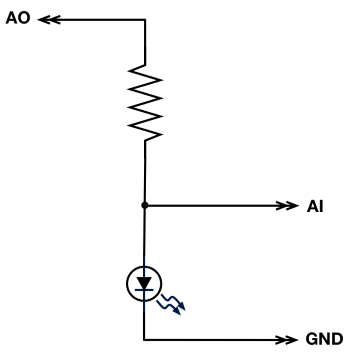
\includegraphics[height=4.4cm]{img/LED_cir.png}};
  \node[black!70] at (5.0,1.0) {LED\_cir.png};
  % gráfica XY
  \node[anchor=south west,black!80] at (8.0,6.2) {XY Graph};
  \begin{scope}[shift={(8.5,0.25)}]
  \begin{axis}[width=7.6cm,height=6.45cm,
    axis background/.style={fill=black!88},
    xmin=-5,xmax=2.5,ymin=-0.2,ymax=3.6,
    grid=major,grid style={green!35!black,line width=.3pt},
    xlabel={\sffamily VD (V)},ylabel={\sffamily ID (mA)},
    label style={font=\sffamily\scriptsize},
    tick label style={font=\sffamily\tiny},
    scaled y ticks=false,
    yticklabel={\pgfmathprintnumber[fixed,fixed zerofill,precision=1]{\tick}E+0},
    axis line style={gray},tick style={gray}]
    \addplot[white,mark=*,mark size=.8pt,thin] table[x=VD,y=ID]{datos/iv_rojo.dat};
  \end{axis}
  \end{scope}
\end{tikzpicture}

  \caption{Esquema del panel frontal del instrumento virtual: controles de la
  rampa ($V_{\text{start}}$, $V_{\text{end}}$, \# muestras), valor de $R$,
  ruta del fichero, imagen del circuito y gráfica $XY$ con $\ID$ (mA, formato
  científico) frente a $\VD$ (V). La curva mostrada corresponde a un LED rojo.}
  \label{fig:panel}
\end{figure}

\subsection{Diagrama de bloques}

\Cref{fig:bloques} resume la lógica del programa. Los puntos que hay que
configurar con cuidado son:

\begin{enumerate}
  \item \textbf{Rampa.} \ttt{Ramp Pattern} genera un vector de \# muestras
    valores equiespaciados entre $V_{\text{start}}$ y $V_{\text{end}}$. El
    vector entra en el bucle \ttt{For} con \emph{auto-indexado}: en cada
    iteración se toma un valor de $\Vin$ y el bucle se repite tantas veces
    como elementos.
  \item \textbf{Temporización.} \ttt{Wait Until Next ms Multiple} con
    \SI{100}{ms} fija el ritmo: una medida cada \SI{0.1}{s} (un barrido de
    100 puntos dura \SI{\approx10}{s}) y da tiempo a que el circuito se
    estabilice.
  \item \textbf{DAQ Assistant de salida (AO-0).}
    \ruta{Generate Signals\,$\to$\,Analog Output\,$\to$\,Voltage\,$\to$\,ao0},
    rango $V_{\min}=\SI{-5}{V}$, $V_{\max}=\SI{5}{V}$, temporización
    \ttt{1 Sample (On Demand)}.
  \item \textbf{DAQ Assistant de entrada (AI-1).}
    \ruta{Acquire Signals\,$\to$\,Analog Input\,$\to$\,Voltage\,$\to$\,ai1},
    rango $\pm\SI{5}{V}$, \ttt{1 Sample (On Demand)}: una lectura de $\VD$ por
    iteración, \emph{después} de escribir $\Vin$.
  \item \textbf{Corriente.} Con funciones aritméticas,
    $\ID\,(\si{mA})=(\Vin-\VD)/R$ con $R$ en k$\Omega$, ec.~\eqref{eq:ohm}.
  \item \textbf{Gráfica.} \ttt{Build XY Graph} con $X=\VD$ e $Y=\ID$;
    desactivad \ttt{Clear data on each call} (doble clic) para que los puntos
    se acumulen, y poned el eje $Y$ en formato científico.
  \item \textbf{Línea de errores.} Encadenad el \emph{error cluster} entre
    los DAQ Assistant: fuerza el orden \emph{escribir}\,$\to$\,\emph{leer} y
    detiene la ejecución si algo falla.
  \item \textbf{Reinicio.} Tras el bucle, un tercer DAQ Assistant (copia del
    de AO-0) escribe \SI{0}{V}, para no dejar el diodo polarizado.
  \item \textbf{Guardado.} \ruta{Programming\,$\to$\,File I/O\,$\to$\,Write
    to Spreadsheet File} con formato \ttt{\%.4e}, la opción
    \ttt{transpose} activada (datos en columnas) y un control de ruta de
    fichero. Guardad al menos las columnas $\Vin$, $\VD$, $\ID$.
\end{enumerate}

\begin{figure}[htbp]
  \centering
  % Diagrama de bloques simplificado del VI (estilo LabVIEW)
\begin{tikzpicture}[font=\sffamily\scriptsize,
  vi/.style={draw=#1!70!black,fill=#1!12,thick,rounded corners=2pt,align=center,
     minimum height=0.95cm,inner sep=3pt},
  vi/.default=azul,
  ctrl/.style={draw=ambar!80!black,fill=ambar!15,thick,align=center,minimum height=0.5cm,
     inner sep=2pt},
  dato/.style={Orange!85!black,line width=1.6pt,-{Stealth[length=5pt]}},
  datov/.style={Orange!85!black,line width=2.6pt,double=white,double distance=.8pt,
     -{Stealth[length=7pt]}},
  err/.style={Goldenrod!70!black,line width=1.2pt,densely dashed,-{Stealth[length=5pt]}}]
  % controles de la rampa
  \node[ctrl] (vs) at (0,2.2) {V start};
  \node[ctrl] (ve) at (0,1.4) {V end};
  \node[ctrl] (nm) at (0,0.6) {\# muestras};
  \node[vi=navy,minimum width=1.7cm] (ramp) at (2.4,1.4) {Ramp\\Pattern};
  \draw[dato] (vs.east) -- ++(0.35,0) |- ([yshift=6pt]ramp.west);
  \draw[dato] (ve.east) -- (ramp.west);
  \draw[dato] (nm.east) -- ++(0.35,0) |- ([yshift=-6pt]ramp.west);
  % bucle for
  \draw[gray!60,line width=4pt,rounded corners=1pt] (3.9,-1.6) rectangle (13.0,3.4);
  \node[draw=gray!60,fill=white,thick,minimum size=0.4cm,font=\sffamily\scriptsize\bfseries,
     inner sep=1pt] at (4.25,3.05) {N};
  \node[draw=gray!60,fill=white,thick,minimum size=0.4cm,font=\sffamily\scriptsize\bfseries,
     inner sep=1pt] at (4.25,-1.25) {i};
  \node[gray!60!black,font=\sffamily\scriptsize\bfseries,anchor=south east] at (13.0,3.55) {bucle For};
  % túnel de auto-indexado
  \node[draw=Orange!85!black,fill=white,minimum size=0.28cm,inner sep=0pt] (tun) at (3.9,1.4) {};
  \draw[Orange!85!black,thick] ([xshift=-2pt]tun.center) -- ([xshift=2pt]tun.center)
     ([yshift=-2pt]tun.center) -- ([yshift=2pt]tun.center);
  \draw[datov] (ramp.east) -- (tun.west);
  % bloques internos
  \node[vi,minimum width=2.2cm] (ao) at (6.0,1.4) {DAQ Assistant\\\textbf{AO-0}: escribe $\Vin$};
  \node[vi,minimum width=2.2cm] (ai) at (6.0,-0.4) {DAQ Assistant\\\textbf{AI-1}: lee $\VD$};
  \node[vi=cVerde,minimum width=2.0cm] (ohm) at (8.9,0.5) {$\ID=\dfrac{\Vin-\VD}{R}$};
  \node[ctrl] (r) at (8.9,2.25) {R (k$\Omega$)};
  \node[vi=navy,minimum width=1.8cm] (xy) at (11.6,0.5) {Build\\XY Graph};
  \node[vi=grisazul,minimum width=1.6cm,minimum height=0.7cm] (wait) at (11.6,2.45)
     {\raisebox{-1pt}{\tikz{\draw[thick](0,0) circle (.12);\draw(0,0)--(0,.09)(0,0)--(.07,0);}}\ Wait until\\ next ms: 100};
  \draw[dato] (tun.east) -- node[above,black!70]{$\Vin$} (ao.west);
  \draw[dato] ($(tun.east)+(0.4,0)$) |- ([yshift=8pt]ohm.west);
  \fill[Orange!85!black] ($(tun.east)+(0.4,0)$) circle (2pt);
  \draw[dato] (ai.east) -- node[below,black!70]{$\VD$} ++(0.6,0) |- ([yshift=-8pt]ohm.west);
  \draw[dato] (r.south) -- (ohm.north);
  \draw[dato] (ohm.east) -- node[above,black!70]{$\ID$} (xy.west);
  \draw[dato] ($(ai.east)+(0.6,0)$) -- ++(0,-0.75) -| ([xshift=-6pt]xy.south);
  \fill[Orange!85!black] ($(ai.east)+(0.6,0)$) circle (2pt);
  \draw[err] (ao.south) -- node[left,Goldenrod!60!black,font=\sffamily\tiny]{error} (ai.north);
  % fuera del bucle
  \node[draw=gray!60,fill=black!85,text=white,minimum width=1.6cm,minimum height=0.9cm,
     align=center] (graf) at (14.6,0.5) {XY\\Graph};
  \draw[dato] (xy.east) -- (graf.west);
  \node[vi,minimum width=2.4cm] (ao0) at (8.0,-2.75) {DAQ Assistant\\\textbf{AO-0} $=\SI{0}{V}$};
  \node[vi=cVerde,minimum width=2.6cm] (file) at (12.0,-2.75) {Write to\\Spreadsheet File\\[-1pt]{\tiny \%.4e, transpose}};
  \draw[err] (ai.south) -- ++(0,-0.75) -| (6.3,-2.75) -- (ao0.west);
  \draw[datov] ([xshift=6pt]xy.south) |- ++(0,-1.2) -| (file.north);
  \node[ctrl] (path) at (14.6,-2.75) {ruta};
  \draw[dato] (path.west) -- (file.east);
\end{tikzpicture}

  \caption{Diagrama de bloques simplificado del instrumento virtual. Las
  líneas naranjas son datos numéricos; la línea discontinua ocre es el
  \emph{error cluster}, que impone el orden de ejecución. El bucle \ttt{For}
  (marco gris) se ejecuta una vez por cada valor de la rampa.}
  \label{fig:bloques}
\end{figure}

\begin{observacion}[Por qué «1 Sample (On Demand)»]
  No queremos generar una forma de onda continua sino un \emph{escalón} por
  iteración: imponer un valor de $\Vin$, esperar a que el circuito se
  estabilice y medir. Es un barrido \emph{cuasiestático}: cada punto
  $(\VD,\ID)$ es un estado estacionario, como en un trazador de curvas
  comercial, y la característica obtenida no depende de la velocidad de
  barrido (a diferencia de un osciloscopio en modo $XY$ con una señal
  triangular rápida, en el que aparecerían efectos capacitivos).
\end{observacion}

% =====================================================================
\section{Lo que veremos en la gráfica}
\label{sec:grafica}
% =====================================================================

Las figuras de esta sección se han obtenido \emph{simulando} el experimento
(ecuación de Shockley con resistencia serie, $R=\SI{1}{k\ohm}$, rampa de
$-5$ a $\SI{5}{V}$ en 101 pasos y ruido de \SI{1}{mV} en AI-1): muestran el
aspecto esperado, pero los valores numéricos de vuestros diodos serán
distintos.

\subsection{Evolución temporal del barrido}

Antes de la gráfica $XY$ conviene entender qué ocurre iteración a iteración
(\cref{fig:temporal}). Mientras el diodo no conduce, $\ID\simeq0$ y no cae
tensión en $R$, luego $\VD\simeq\Vin$: la tensión medida \emph{sigue} a la
impuesta. Al alcanzar el umbral, $\VD$ se \emph{satura} en $\approx\Vg$ y todo
el exceso $\Vin-\Vg$ cae en $R$: la corriente crece linealmente con el índice
de la muestra.

\begin{figure}[htbp]
  \centering
  % Evolución temporal del barrido para un LED rojo
\begin{tikzpicture}
\begin{groupplot}[group style={group size=1 by 2,vertical sep=0.35cm,
    xticklabels at=edge bottom},
  width=0.88\linewidth,xmin=0,xmax=100,grid=major,
  legend pos=north west,legend cell align=left]
  \nextgroupplot[height=5.0cm,ylabel={Tensión (V)},ymin=-5.5,ymax=5.5]
    \fill[azulclaro,opacity=.7] (axis cs:68,-5.5) rectangle (axis cs:100,5.5);
    \addplot[grisazul,thick,mark=none] table[x=k,y=Vin]{datos/iv_rojo.dat};
    \addlegendentry{$\Vin$ (AO-0)}
    \addplot[cRojo,mark=*,mark size=1pt,only marks] table[x=k,y=VD]{datos/iv_rojo.dat};
    \addlegendentry{$\VD$ (AI-1)}
    \node[font=\scriptsize,azul,anchor=north] at (axis cs:84,-1.2) {LED en conducción};
    \node[font=\scriptsize,grisazul,anchor=south] at (axis cs:30,0.2) {$\VD\simeq\Vin$ (corte)};
    \draw[rojoaviso,densely dashed] (axis cs:0,1.77) -- (axis cs:100,1.77)
      node[pos=0.08,above,font=\scriptsize]{$\Vg$};
  \nextgroupplot[height=3.6cm,ylabel={$\ID$ (mA)},xlabel={Índice de muestra $k$},
    ymin=-0.4,ymax=3.6]
    \fill[azulclaro,opacity=.7] (axis cs:68,-0.4) rectangle (axis cs:100,3.6);
    \addplot[navy,mark=*,mark size=1pt,only marks] table[x=k,y=ID]{datos/iv_rojo.dat};
    \node[font=\scriptsize,navy,anchor=west] at (axis cs:3,1.9)
      {$\ID=(\Vin-\VD)/R$};
\end{groupplot}
\end{tikzpicture}

  \caption{Barrido de un LED rojo en función del índice de muestra $k$
  (cada \SI{100}{ms}). Arriba: tensión impuesta $\Vin$ y medida $\VD$; por
  encima del umbral $\VD$ queda anclada en $\approx\SI{1.8}{V}$. Abajo:
  corriente calculada, nula hasta el umbral y después
  $\ID\simeq(\Vin-\Vg)/R$.}
  \label{fig:temporal}
\end{figure}

\subsection{Diodo pn y diodo Zener}

\begin{figure}[htbp]
  \centering
  % Características I-V del diodo pn y del Zener
\begin{tikzpicture}
\begin{groupplot}[group style={group size=2 by 1,horizontal sep=1.5cm},
  width=0.53\linewidth,height=6.4cm,xmin=-5.3,xmax=1.3,
  xlabel={$\VD$ (V)},grid=major,legend pos=north west,legend cell align=left]
  % ---------- (a) pn
  \nextgroupplot[ylabel={$\ID$ (mA)},ymin=-2.2,ymax=4.8,title={(a) Diodo pn (Si)},
     title style={font=\small\color{navy}}]
    \addplot[medida,cPN] table[x=VD,y=ID]{datos/iv_pn.dat};
    \addlegendentry{datos}
    \addplot[azul,dashed,thick] table[x=VD,y=ID]{datos/fit_pn.dat};
    \addlegendentry{extrapolación}
    \fill[rojoaviso] (axis cs:\umbralpn,0) circle (1.8pt);
    \node[rojoaviso,font=\scriptsize,anchor=north west] at (axis cs:0.2,-0.15) {$\Vg$};
    \node[font=\scriptsize,grisazul,align=center] at (axis cs:-2.6,-0.75)
      {corte: $\ID\simeq0$, $\VD=\Vin$};
  % ---------- (b) Zener
  \nextgroupplot[ymin=-2.2,ymax=4.8,title={(b) Diodo Zener ($\VZ$ nominal \SI{3.3}{V})},
     title style={font=\small\color{navy}}]
    \addplot[medida,cZener] table[x=VD,y=ID]{datos/iv_zener.dat};
    \addlegendentry{datos}
    \addplot[azul,dashed,thick,forget plot] table[x=VD,y=ID]{datos/fit_zener.dat};
    \addplot[azul,dashed,thick] table[x=VD,y=ID]{datos/fitz_zener.dat};
    \addlegendentry{extrapolación}
    \fill[rojoaviso] (axis cs:\umbralzener,0) circle (1.8pt);
    \fill[rojoaviso] (axis cs:-\tensionzener,0) circle (1.8pt);
    \node[rojoaviso,font=\scriptsize,anchor=south east] at (axis cs:\umbralzener,0.1) {$\Vg$};
    \node[rojoaviso,font=\scriptsize,anchor=south west] at (axis cs:-\tensionzener,0.1) {$-\VZ$};
    \node[font=\scriptsize,grisazul,align=center,anchor=north] at (axis cs:-1.4,-0.9)
      {ruptura: $\VD\simeq-\VZ$};
\end{groupplot}
\end{tikzpicture}

  \caption{Características $\ID(\VD)$ simuladas. (a) Diodo pn de Si: en
  inversa $\ID\simeq0$ en todo el rango; en directa conduce a partir de
  $\Vg\simeq\SI{\umbralpn}{V}$. (b) Diodo Zener de \SI{3.3}{V}: en directa se
  comporta como el pn ($\Vg\simeq\SI{\umbralzener}{V}$); en inversa entra en
  ruptura y $\VD$ queda fija en $-\VZ$, con $\VZ\simeq\SI{\tensionzener}{V}$
  obtenida extrapolando la rama inversa.}
  \label{fig:pn-zener}
\end{figure}

En la gráfica $XY$ (\cref{fig:pn-zener}) se reconocen las regiones de la
característica:
\begin{enumerate}
  \item \textbf{Corte (inversa)}: puntos sobre el eje $\ID=0$, igualmente
    espaciados en $\VD$ porque $\VD=\Vin$.
  \item \textbf{Codo}: transición en torno a $\Vg$.
  \item \textbf{Conducción}: rama casi vertical; los puntos se reparten
    uniformemente \emph{en corriente} (paso $\Delta\Vin/R$) y se apiñan en
    tensión.
  \item \textbf{Ruptura} (solo Zener): rama vertical en $\VD=-\VZ$, con
    corriente negativa $(\Vin+\VZ)/R$.
\end{enumerate}

\subsection{LED de distintos colores}

\begin{figure}[htbp]
  \centering
  % Características I-V de los siete LED
\begin{tikzpicture}
\begin{axis}[width=\linewidth,height=8.2cm,
  xmin=-1.2,xmax=3.4,ymin=-0.25,ymax=4.1,
  xlabel={$\VD$ (V)},ylabel={$\ID$ (mA)},grid=major,
  legend pos=north west,legend cell align=left,legend columns=1]
  \foreach \col/\fic/\n in {cIR/ir/IR\ (940\,nm),cRojo/rojo/Rojo\ (630\,nm),
      cAmarillo/amarillo/Amarillo\ (590\,nm),cVerde/verde/Verde\ (525\,nm),
      cAzul/azul/Azul\ (470\,nm),cBlanco/blanco/Blanco,cUV/uv/UV\ (400\,nm)}{
    \edef\temp{\noexpand\addplot[\col,mark=*,mark size=1.2pt,only marks]
      table[x=VD,y=ID]{datos/iv_\fic.dat};
      \noexpand\addlegendentry{\n}
      \noexpand\addplot[\col,dashed,forget plot] table[x=VD,y=ID]{datos/fit_\fic.dat};}
    \temp}
  \draw[black!50] (axis cs:-1.2,0) -- (axis cs:3.4,0);
  \draw[-{Stealth[length=6pt]},navy,thick] (axis cs:1.2,3.75) -- (axis cs:2.85,3.75)
    node[midway,above,font=\scriptsize]{$\lambda$ decreciente $\Rightarrow$ $\Vg$ creciente};
\end{axis}
\end{tikzpicture}

  \caption{Características $\ID(\VD)$ simuladas de los siete LED, con las
  rectas de extrapolación (discontinuas) que definen $\Vg$. El umbral se
  desplaza hacia la derecha al disminuir $\lambda$: IR $<$ rojo $<$ amarillo
  $<$ verde $<$ azul $\approx$ blanco $<$ UV. Como $I_{\max}=(\SI{5}{V}-\Vg)/R$,
  los LED de umbral alto alcanzan menos corriente.}
  \label{fig:leds}
\end{figure}

La \cref{fig:leds} es la gráfica principal del informe. Al ejecutar el
programa, observad además a qué corriente empieza a verse luz: los LED
modernos son visibles con decenas de $\si{\micro A}$, es decir, ya en el codo.
El LED IR no se ve a simple vista, pero sí con la cámara de un teléfono.

\begin{observacion}[Lo que \emph{no} veremos]
  En inversa los LED no entran en ruptura con $|\VD|\le\SI{5}{V}$ (su
  tensión inversa máxima suele ser \SI{5}{V}): la rama negativa será plana. Si
  alguna curva aparece «al revés» o con $\VD$ siempre igual a $\Vin$, el LED
  está invertido o el circuito abierto.
\end{observacion}

% =====================================================================
\section{Análisis de los datos}
\label{sec:analisis}
% =====================================================================

\subsection{Extracción de la tensión umbral y de la tensión Zener}

\begin{laboratorio}{Procedimiento recomendado}{procedimiento}
  \begin{enumerate}[leftmargin=2em]
    \item Cargad el fichero (columnas $\Vin$, $\VD$, $\ID$) y representad
      $\ID$ frente a $\VD$ con puntos, sin unirlos.
    \item Seleccionad el tramo de alta corriente, por ejemplo
      $\ID>I_{\max}/2$, y ajustad una recta $\ID=a\VD+b$ por mínimos
      cuadrados.
    \item La tensión umbral es la intersección con el eje: $\Vg=-b/a$. Su
      incertidumbre se obtiene propagando las de $a$ y $b$ (incluyendo su
      covarianza).
    \item Para el Zener, repetid el ajuste en la rama inversa de alta corriente
      ($\ID<I_{\min}/2$): $\VZ=b/a$ con el signo adecuado.
    \item Indicad siempre el criterio usado: otros criterios (p.\,ej.\
      $\Vg=\VD$ a $\ID=\SI{0.1}{mA}$) dan valores algo distintos.
  \end{enumerate}
\end{laboratorio}

\begin{observacion}[Fuentes de incertidumbre]
  La resolución de AI-1 (16 bits) y su ruido ($\sim$\SI{1}{mV}) apenas afectan
  a $\VD$; la tolerancia de $R$ (5\,\%) escala $\ID$ pero no desplaza la
  intersección con $\ID=0$. Lo que más influye es la \emph{elección del tramo}
  de ajuste y la temperatura del diodo. Medid el valor real de $R$ con el
  multímetro e introducidlo en el panel.
\end{observacion}

\subsection{Umbral frente a energía del fotón: estimación de \texorpdfstring{$h$}{h}}
\label{sec:planck}

Según~\eqref{eq:umbral-lambda}, representando $\Vg$ frente a
$E_{\text{ph}}=hc/\lambda_p$ (en eV) los puntos deben alinearse sobre una
recta de pendiente próxima a~1 (\cref{fig:planck}); equivalentemente, cada LED
da una estimación de la constante de Planck,
\begin{destacada}
  h\simeq\frac{e\,\Vg\,\lambda_p}{c},
  \label{eq:planck}
\end{destacada}
que con los datos simulados de la \cref{tab:resultados} sale entre
$5{,}5$ y $\SI{7e-34}{J.s}$ (valor exacto: $\SI{6.626e-34}{J.s}$). La dispersión
refleja las limitaciones comentadas en la observación~\ref{obs:desv}.

\begin{figure}[htbp]
  \centering
  % Tensión umbral frente a energía del fotón
\begin{tikzpicture}
\begin{axis}[width=0.82\linewidth,height=6.8cm,
  xmin=1.1,xmax=3.4,ymin=0.8,ymax=3.4,
  xlabel={Energía del fotón $E_{\text{ph}}=hc/\lambda_p$ (eV)},
  ylabel={Tensión umbral $\Vg$ (V)},grid=major,
  legend pos=north west,legend cell align=left]
  \addplot[grisazul,thick,domain=1.1:3.4,samples=2]{x};
  \addlegendentry{ideal, $e\Vg=E_{\text{ph}}$}
  \addplot[azul,dashed,thick] table[x=E,y=Vth]{datos/umbral_fit.dat};
  \addlegendentry{ajuste lineal}
  \foreach \col/\e/\v/\t/\anc in {cIR/1.319/1.10/IR/north west,cRojo/1.968/1.77/rojo/north west,
      cAmarillo/2.101/1.86/amarillo/north west,cVerde/2.362/2.47/verde/south east,
      cAzul/2.638/2.59/azul/north,cUV/3.100/2.97/UV/north west}{
    \edef\temp{\noexpand\addplot[only marks,mark=*,mark size=3pt,\col,
       draw=black!60,forget plot] coordinates {(\e,\v)};
       \noexpand\node[font=\noexpand\scriptsize,\col,anchor=\anc] at (axis cs:\e,\v) {\t};}
    \temp}
  \addplot[only marks,mark=o,mark size=3pt,cBlanco,thick,forget plot] coordinates {(2.725,2.63)};
  \node[font=\scriptsize,cBlanco,anchor=north west] at (axis cs:2.74,2.6) {blanco};
\end{axis}
\end{tikzpicture}

  \caption{Tensión umbral (datos simulados) frente a la energía del fotón. La
  línea continua es la relación ideal $e\Vg=E_{\text{ph}}$; la discontinua, el
  ajuste lineal $\Vg=\num{\pendienteajuste}\,E_{\text{ph}}/e\num{\ordenadaajuste}\,\si{V}$
  (sin el LED blanco, cuyo umbral es el de su chip azul).}
  \label{fig:planck}
\end{figure}

\begin{table}[htbp]
  \centering\small
  \caption{Ejemplo de tabla de resultados para el informe (valores
  simulados). $h$ se estima con la ec.~\eqref{eq:planck}.}
  \label{tab:resultados}
  \renewcommand{\arraystretch}{1.15}
  \begin{tabular}{@{}l l c c c c@{}}
    \toprule
    \textbf{LED} & \textbf{Material} & $\lambda_p$ (nm) & $E_{\text{ph}}$ (eV)
      & $\Vg$ (V) & $h$ ($10^{-34}$\,J\,s)\\
    \midrule
    \tablaumbral
    \midrule
    Diodo pn & Si & --- & --- & \num{\umbralpn} & ---\\
    Zener    & Si & --- & --- & \num{\umbralzener}\ ($\VZ=\num{\tensionzener}$) & ---\\
    \bottomrule
  \end{tabular}
\end{table}

% =====================================================================
\section{Lista de comprobación y evaluación}
\label{sec:checklist}
% =====================================================================

\begin{tcolorbox}[enhanced,sharp corners,boxrule=0pt,frame hidden,
  borderline west={2.2pt}{0pt}{navy},lineas=grisclaro,
  interior style={left color=azulclaro,right color=white},left=10pt,right=8pt]
\small\setlist[itemize]{label=\casilla,leftmargin=1.4em,itemsep=1pt,topsep=2pt}
\begin{minipage}[t]{0.48\linewidth}
{\color{navy}\bfseries Montaje}
\begin{itemize}
  \item $R=\SI{1}{k\ohm}$ medida con el multímetro.
  \item Diodo/LED con el ánodo hacia $R$.
  \item AO-0\,$\to$\,$R$; AI-1\,$\to$\,ánodo; GND\,$\to$\,cátodo.
  \item (myDAQ) AI-1\,$-$ a masa.
\end{itemize}
{\color{navy}\bfseries Programa}
\begin{itemize}
  \item Rampa de $-5$ a $\SI{5}{V}$, $N\ge100$.
  \item Espera de \SI{100}{ms} en el bucle.
  \item DAQ en \ttt{1 Sample (On Demand)}, $\pm\SI{5}{V}$.
  \item \ttt{Clear data on each call} desactivado.
  \item AO-0 a \SI{0}{V} al terminar.
  \item Guardado en \ttt{\%.4e}, transpuesto.
\end{itemize}
\end{minipage}\hfill
\begin{minipage}[t]{0.48\linewidth}
{\color{navy}\bfseries Medidas}
\begin{itemize}
  \item Diodo pn.
  \item Diodo Zener (anotar su $\VZ$ nominal).
  \item LED IR, rojo, amarillo, verde, azul, blanco y UV.
  \item Un fichero por componente, con nombre claro.
  \item Anotar $\lambda_p$ de cada LED (hoja de datos).
\end{itemize}
{\color{navy}\bfseries Informe (máx.\ 3 páginas)}
\begin{itemize}
  \item Código subido (uno por grupo, nombres en el panel).
  \item Explicación del panel frontal y del diagrama.
  \item Gráficas $\ID(\VD)$ como las del \cref{sec:grafica}.
  \item $\Vg$ de cada diodo y $\VZ$ del Zener.
  \item Discusión de $\Vg$ frente a color y $\lambda$.
\end{itemize}
\end{minipage}
\end{tcolorbox}

% =====================================================================
\clearpage
\appendix
\section{Formulario}
% =====================================================================

\begin{center}
\renewcommand{\arraystretch}{2.0}
\begin{tabularx}{\linewidth}{@{}>{\raggedright\arraybackslash}p{0.36\linewidth} X@{}}
  \toprule
  Ecuación de Shockley & $\displaystyle \ID=\IS\bigl(e^{\VD/n\VT}-1\bigr),\qquad \VT=\frac{k_BT}{e}\simeq\SI{25.9}{mV}$\\
  Resistencia dinámica & $\displaystyle r_d=\frac{\mathrm d\VD}{\mathrm d\ID}\simeq\frac{n\VT}{\ID}$\\
  Corriente en el circuito & $\displaystyle \ID\,(\si{mA})=\frac{\Vin-\VD}{R\,(\si{k\ohm})}$\\
  Recta de carga & $\displaystyle \ID=\frac{\Vin}{R}-\frac{\VD}{R},\qquad I_{\max}\simeq\frac{\Vin-\Vg}{R}$\\
  Umbral por extrapolación & $\displaystyle \ID\simeq a\VD+b\ \Rightarrow\ \Vg=-\frac{b}{a}$\\
  Color del LED & $\displaystyle \lambda\simeq\frac{hc}{\Eg},\qquad \lambda[\si{nm}]\simeq\frac{1240}{\Eg[\si{eV}]}$\\
  Umbral y longitud de onda & $\displaystyle e\Vg\simeq\frac{hc}{\lambda}\ \Rightarrow\ h\simeq\frac{e\Vg\lambda}{c}$\\
  Constantes & $h=\SI{6.626e-34}{J.s}$,\quad $c=\SI{2.998e8}{m/s}$\\[-8pt]
   & $e=\SI{1.602e-19}{C}$,\quad $k_B=\SI{8.617e-5}{eV/K}$\\
  \bottomrule
\end{tabularx}
\end{center}

% =====================================================================
\begin{thebibliography}{9}
\addcontentsline{toc}{section}{Referencias}
\small
\bibitem{guion} Instrumentación Electrónica, \emph{Práctica \#3:
  Identificación y caracterización de diodos}, Grado en Física, Universidad de
  Salamanca, curso 2026/2027.
\bibitem{sze} S.\,M.~Sze y K.\,K.~Ng, \emph{Physics of Semiconductor Devices},
  3.ª ed., Wiley, 2007.
\bibitem{pierret} R.\,F.~Pierret, \emph{Semiconductor Device Fundamentals},
  Addison-Wesley, 1996.
\bibitem{schubert} E.\,F.~Schubert, \emph{Light-Emitting Diodes}, 2.ª ed.,
  Cambridge University Press, 2006.
\bibitem{horowitz} P.~Horowitz y W.~Hill, \emph{The Art of Electronics},
  3.ª ed., Cambridge University Press, 2015.
\bibitem{sedra} A.\,S.~Sedra y K.\,C.~Smith, \emph{Microelectronic Circuits},
  7.ª ed., Oxford University Press, 2015.
\bibitem{shockley} W.~Shockley, «The theory of p-n junctions in
  semiconductors and p-n junction transistors», \emph{Bell Syst.\ Tech.\ J.}
  \textbf{28}, 435--489 (1949).
\bibitem{mydaq} National Instruments, \emph{NI myDAQ User Guide}.
\end{thebibliography}

\end{document}
